\documentclass[a4paper, oneside]{thesis}

\usepackage[utf8]{inputenc}
\usepackage[T1]{fontenc}
\usepackage{float}

%for including full pdf pages
\usepackage[]{pdfpages} 

%%%%%%%%%%%%%%%%%%%%%%%%%%%%%%%%%%%%%%%%%%%%%%%%%%%%%%%%%%%
% DOCUMENT METADATA

\title{Development of an Interactive Online Learning Environment for Elementary School Students with Focus on Algorithmic Tasks, Based on the Textbook "einfach Informatik 3/4"}
\thesistype{Bachelor's Thesis}

\author{Dario Naepfer}
\email{dnaepfer@student.ethz.ch}

\supervisors{Prof.\ Dr.\ Juraj\ Hromkovič\\Regula\ Lacher\\Dr.\ Elizabeta\ Cavar}

\institute{Chair of Information Technology and Education \\[2pt]
ETH Zürich}

\date{\today}

%%%%%%%%%%%%%%%%%%%%%%%%%%%%%%%%%%%%%%%%%%%%%%%%%%%%%%%%%%%

\begin{document}

\frontmatter % do not remove this line
\maketitle

\cleardoublepage

\begin{abstract}
	This thesis gives an outline of the project and implementation of an online learning environment that teaches important concepts from the \textit{ABZ} textbook 'einfach Informatik 3/4'. This book is about to be published in order to reinforce the emerging focus on the field of IT in elementary school. The implemented task sets of 'einfach Informatik 3/4' deal with the autonomous solving of problems.

The learning environment will be analysed in-depth such that the reader is introduced to the various design choices as well as the architecture of the program. Also, the task concept will be covered and, finally, an assessment of live testing of the learning environment will be exhaustively discussed. 



\end{abstract}

\begin{acknowledgements}
	First of all, I would like to thank \textit{Prof. Dr. Juraj Hromkovic} for the offer to supervise my Bachelor's thesis, for the friendly welcome and uncomplicated procedure, and for the feedback during the thesis. The opportunity given to me was a unique chance to dive into software development and has taught me a lot in various areas of software engineering.

Also, I would like to express my gratitude to \textit{Regula Lacher} as well as \textit{Dr. Elizabeta Cavar} for the ongoing support throughout the project. By their constructive feedback and useful tips, I learned a lot, and it motivated me to keep going. 

Further, my family and friends have helped me a lot with their support, encouragement and feedback, even in providing contacts to test the project in different elementary schools and testing the environment themselves. I'm very thankful for each one of them.

Last but not least, special thanks are given to the proofreaders \textit{Esther Naepfer} and \textit{Markus Naepfer}.
\end{acknowledgements}

{
  \hypersetup{linkcolor=black}
  \tableofcontents
}

\mainmatter % do not remove this line

% Start writing here
\chapter{Introduction}

\section{Background and Motivation}

Over the course of the past years, computer science has become significantly more important not only in the academic world, but also in all of modern society. In Switzerland, the introduction of Lehrplan 21 \cite{Lehrplan21} accelerated this process. In order to cope with these changes, the Center for Computer Science Education at ETH Zurich (also known as ABZ \cite{ABZ}) has set itself the target to support the introduction of computer science as one of the foundation subjects in the obligatory school curricula. 

ABZ has been publishing educational material such as textbooks, courses and online platforms. The purpose is to bring computer science into classrooms such that basic computer science concepts may be familiarized among teen pupil. In particular, the disciples will be playfully introduced into topics such as information and data handling, encryption, the finding of strategies and application of algorithms.


\section{Objectives}

The main objective of the thesis is the design, implementation, and testing of tasks in an online learning environment. Content-wise, the tasks will consist of problems and activities proposed in chapter II “Probleme lösen” of the ABZ textbook “einfach Informatik 3/4” that covers the solving of algorithmic problems. In particular, the simple algorithmic concepts of this chapter will be modelled as tasks that are suitable for elementary school. This newly created learning environment will provide a smooth introduction to latter algorithms using a bottom-up approach such that difficulty increases as the users progress.

The platform is to be deployed in schools and utilized alongside the corresponding ABZ textbook. Thus, it is imperative that this web-based environment is stable and works fluently on common operating systems. Also, it should be suitable for teachers as well as their disciples by providing tasks complementary to the other learning material. The environment will then be embedded into the already existing learning repository of ABZ.

As part of the Bachelor’s Thesis, the student is expected to tackle the problem by solving
three sub-tasks, according to the Bachelor's thesis proposal:

\subsection{Design and Concept of the Tasks and the Environment}
\label{subsection:t1}
For a start, an exhaustive study of the relevant chapters of the new ABZ textbook “einfach Informatik 3/4” needs to be done in order to thoroughly understand the algorithmic concepts and how they can be modelled. Also, the corresponding didactic publications of Chair of Information Technology and Education as well as further literature on teaching methods in computer science should be studied in a way that its concepts can be taken into consideration. Then, the tasks that should be implemented are to be fixed and modelled, and their user interface is to be designed. In addition,
different frameworks should be compared and the details of the implementation need to be fixed.

\subsection{Implementation and Testing of the Environment}
\label{subsection:t2}
As a next step, the before-hand modelled tasks will be implemented. In order to do this, the technical programming concepts and languages have to be examined and understood. Furthermore, the code to be implemented should be consistent with the above-mentioned design and concept. The environment will finally be tested under various circumstances and a report is made.

\subsection{Presentation of the Results}
\label{subsection:t3}
At the end, the procedure will be documented in a comprehensive report. Not only the thesis but also the environment will be explained and demonstrated in a concluding presentation.

\newpage
\section{Thesis Outline}
This report will describe the implementation project in detail, starting with its design choices and consequences thereof. Then, the general architecture of the environment will be presented, including details of the program user interface. In the latter section, important components for the build-up of the environment will be discussed. Next, the general task concept will be laid out. Then, for each task set, some remarkable implementation features will be focused on more closely. Before drawing a conclusion, this report also features the results and the experience of live testing of the learning environment in different age groups.


%The source code, live testing results, this report and all other used scripts and documents can be found on the ETH GitLab at \url{https://gitlab.ethz.ch/dnaepfer/bsc-thesis}.
\chapter{Design Choices}
\label{chapter:design}

\section{Introduction}
\label{section:introduction}
For a start, the design of the learning environment will be investigated more closely. First, the two possibilities for the main implementation structure will be presented. Then, the decisions of less general implementation techniques will be pointed out, and lastly, some graphical design details will be taken into consideration.

\section{Design Research}
\label{section:designchoice}
Before the project was launched, some research had to be done such as the acquisition of knowledge and implementation techniques in order to avoid common mistakes. Planning is a fundamental step in building a successful learning environment. The most general choices that have to be made in the beginning can support the creation of different exercises or features or heavily handicap this process. The research that had to be done included the following topics, listed in descending order, starting from the most fundamental and general choice: 

\begin{itemize}
\item Choice of the web framework
\item Choice of the underlying programming language
\item Choice of the graphical user interface (GUI)
\item Choice of the technical structure of the learning environment
\item Choice of the practical structure of the learning environment
\item Choice of the graphical design
\end{itemize}
In the following, the design choices based on research results will be presented. This will help to understand the general structure of the project and lays the foundation to understand the learning environment architecture in the following chapter.

\section{Choice of the Web Framework}
\label{section:designchoice}
In the beginning of the project, major decisions on how to design and implement the learning environment were to be taken. At ABZ, there were already several learning environments in use when this project was about to start. One major requirement of the newly created environment was that it can be embedded or connected with an already existing environment. As a first step, research on these already existing platforms had to be done. This included meetings with programmers and maintenance personnel, as well as technical research on implementation options and techniques was carried out. 

Other learning environments from ETH \cite{L1} and private organizations were analysed as inspiration for the design and functionality. For example, the online platform called Hamsterkiste \cite{L2} and an even bigger environment with name Schlaukopf \cite{L3} were taken into consideration. Soon, two options emerged that could be considered realistic and reasonable. The two options will be examined more closely in the following sections.

\subsection{Option 1}
One possibility to move on was to embed the newly created platform into the already existing programming environment from ABZ \cite{SBT}. Within this given framework, new tasks can be created and added. The functionality and design choices of this framework are, however, restrictive. The design of the task is fixed and the scope of new functions is heavily limited  (see examples in figures \ref{fig:P11} and  \ref{fig:P12}). 


\begin{figure}[H]
    \centering
    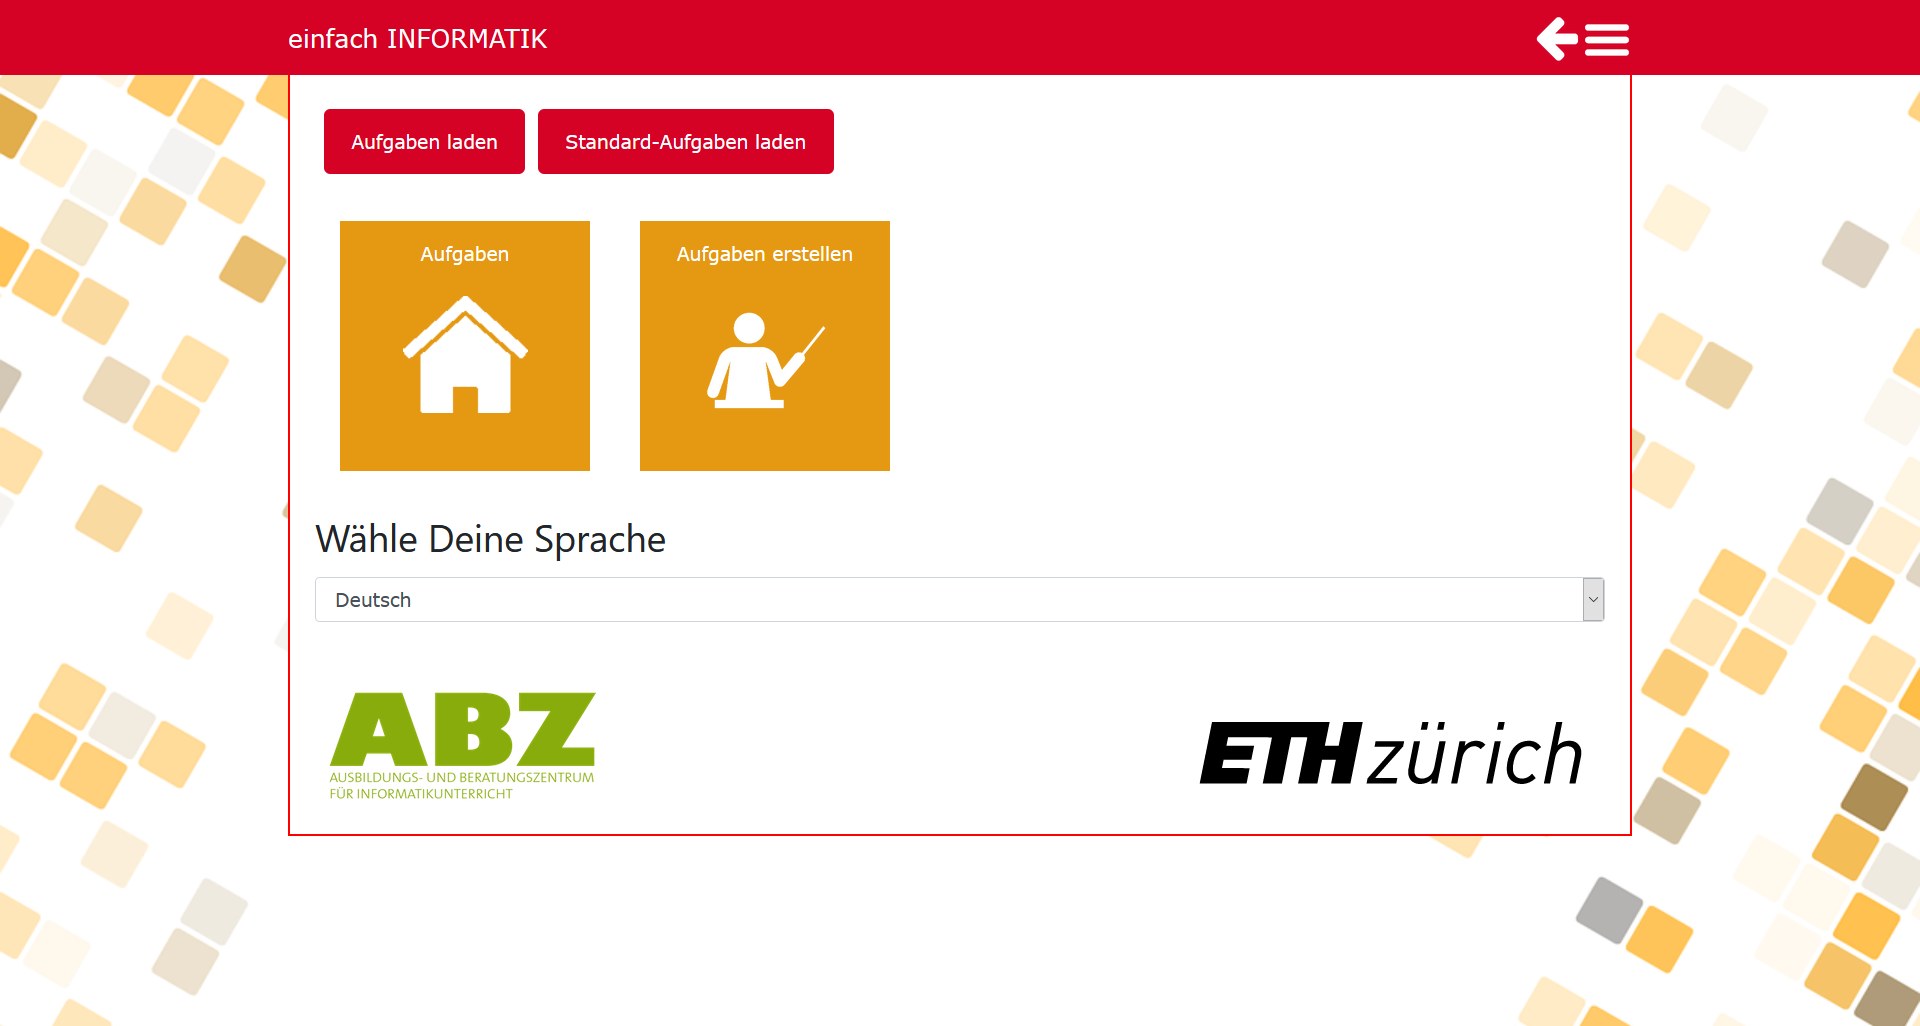
\includegraphics[width=1.0\columnwidth]{figures/P12.png}
    \caption{Home Page of Option 1}
    \label{fig:P11} 
\end{figure}

\begin{figure}[H]
    \centering
    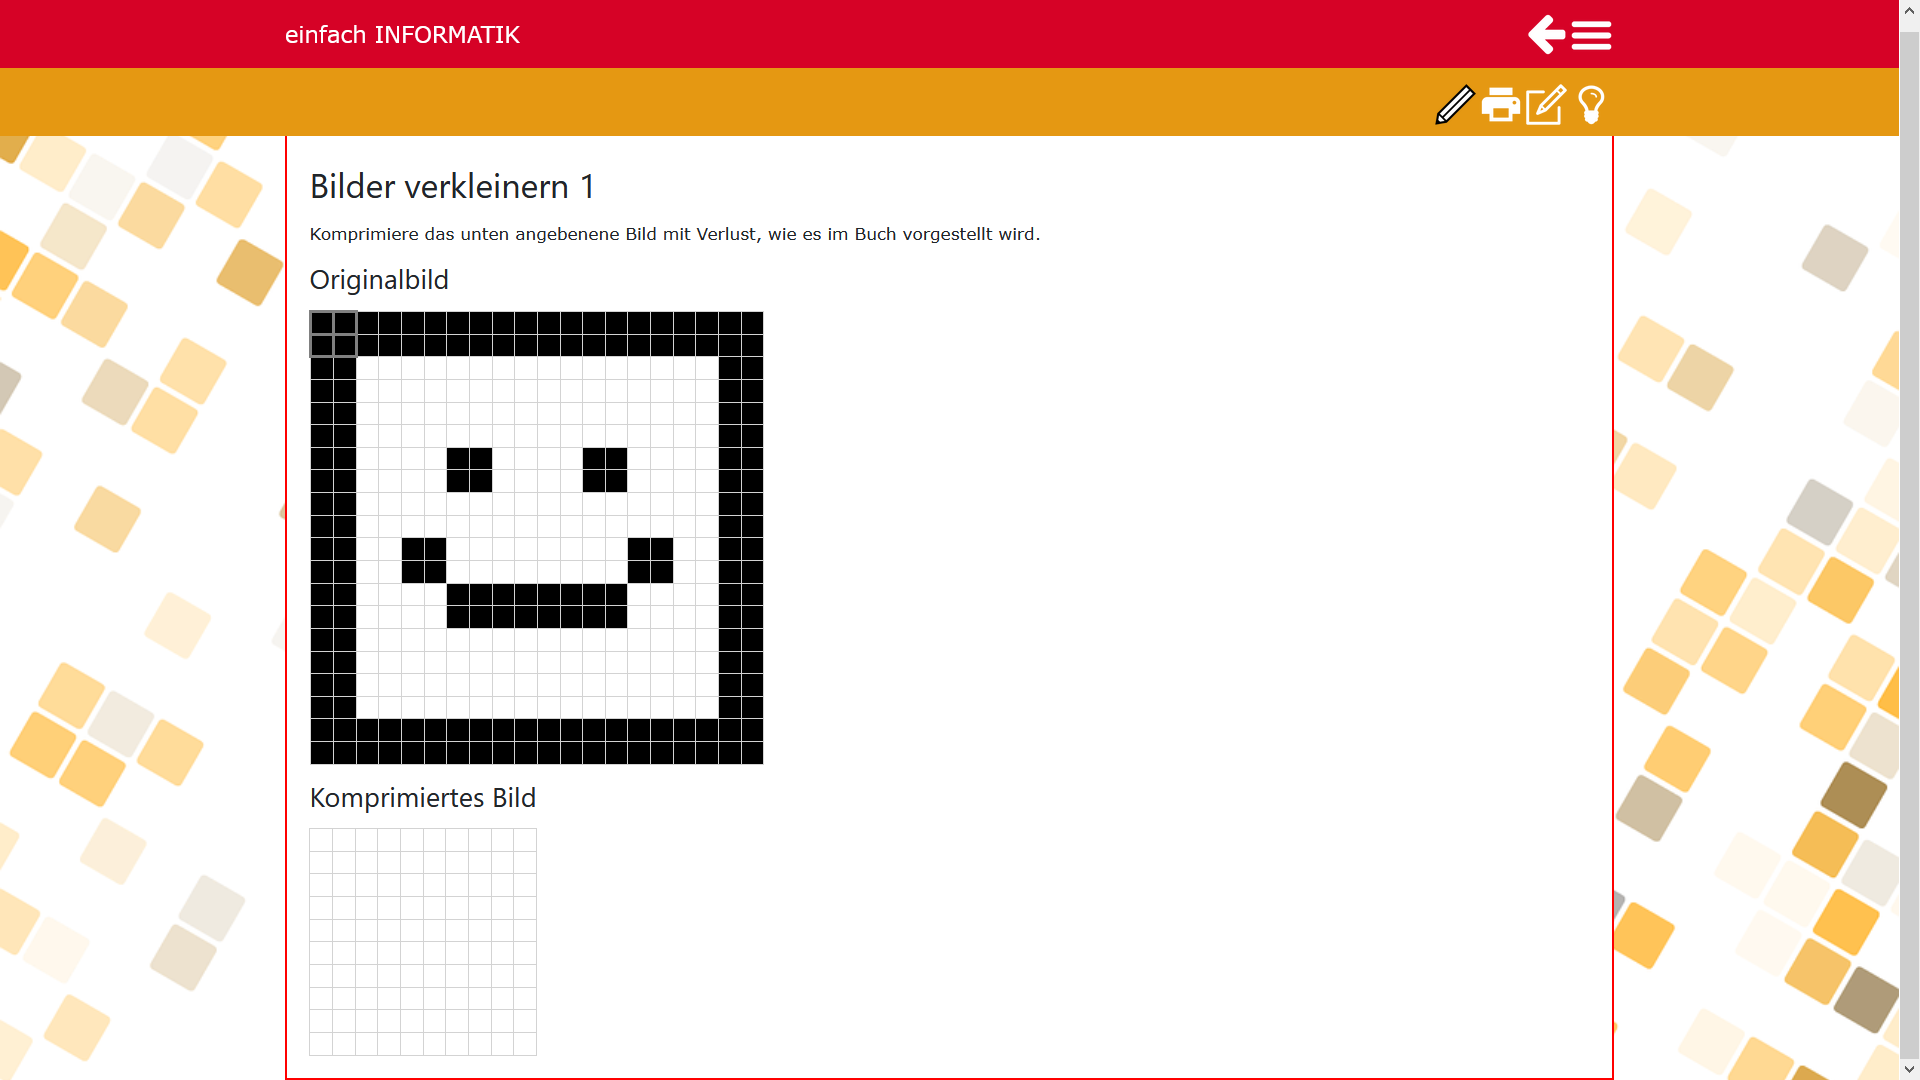
\includegraphics[width=1.0\columnwidth]{figures/P11.png}
    \caption{In-Game Snapshot of Option 1}
    \label{fig:P12} 
\end{figure}

\newpage
\subsection{Option 2}
The alternative to embedding the project into ABZ's framework was to create a new environment from scratch that then can easily be connected with the other environments for "einfach Informatik 3/4" that are about to emerge. The advantage of this choice is that a new project for the age group of third and fourth grade has been successfully completed and launched \cite{FBBT}. This project is more user-friendly and better adapted to the age group (see figures \ref{fig:P21} and  \ref{fig:P22}).

\begin{figure}[H]
    \centering
    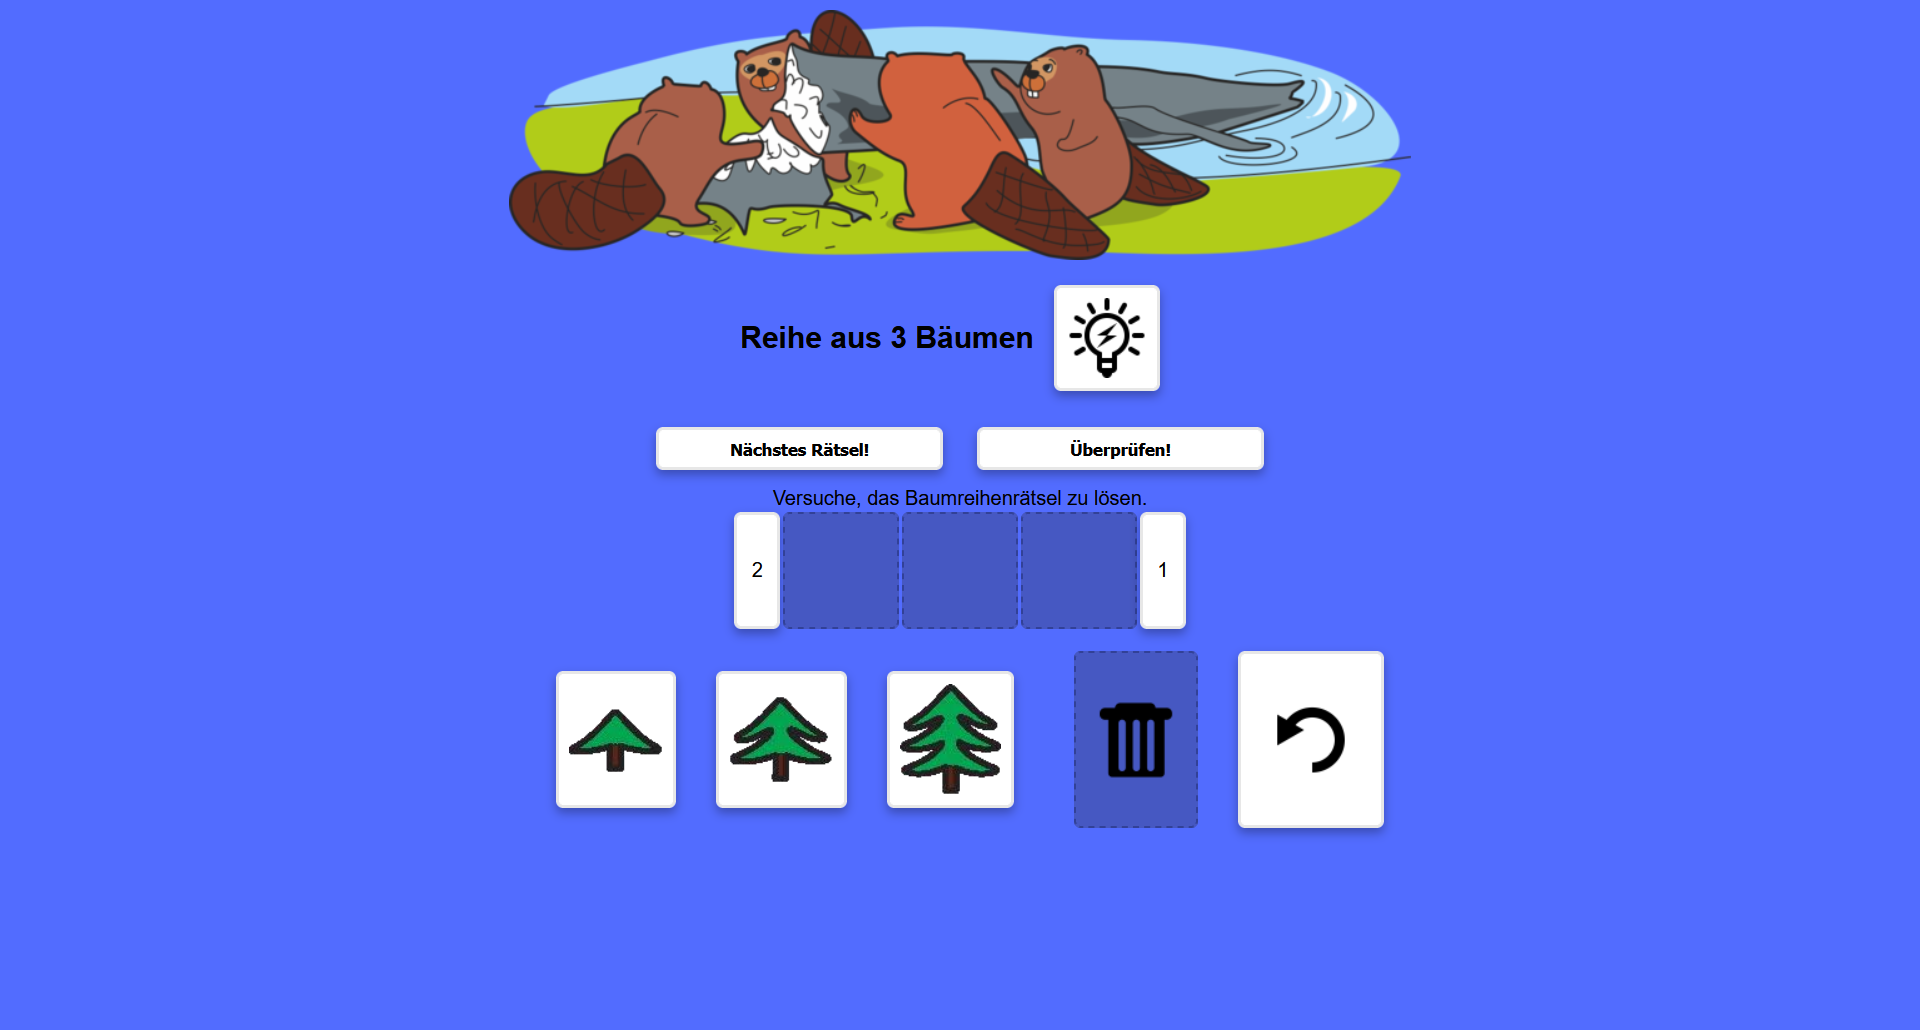
\includegraphics[width=1.0\columnwidth]{figures/P21.png}
    \caption{Home Page of Option 2}
    \label{fig:P21} 
\end{figure}

\begin{figure}[H]
    \centering
    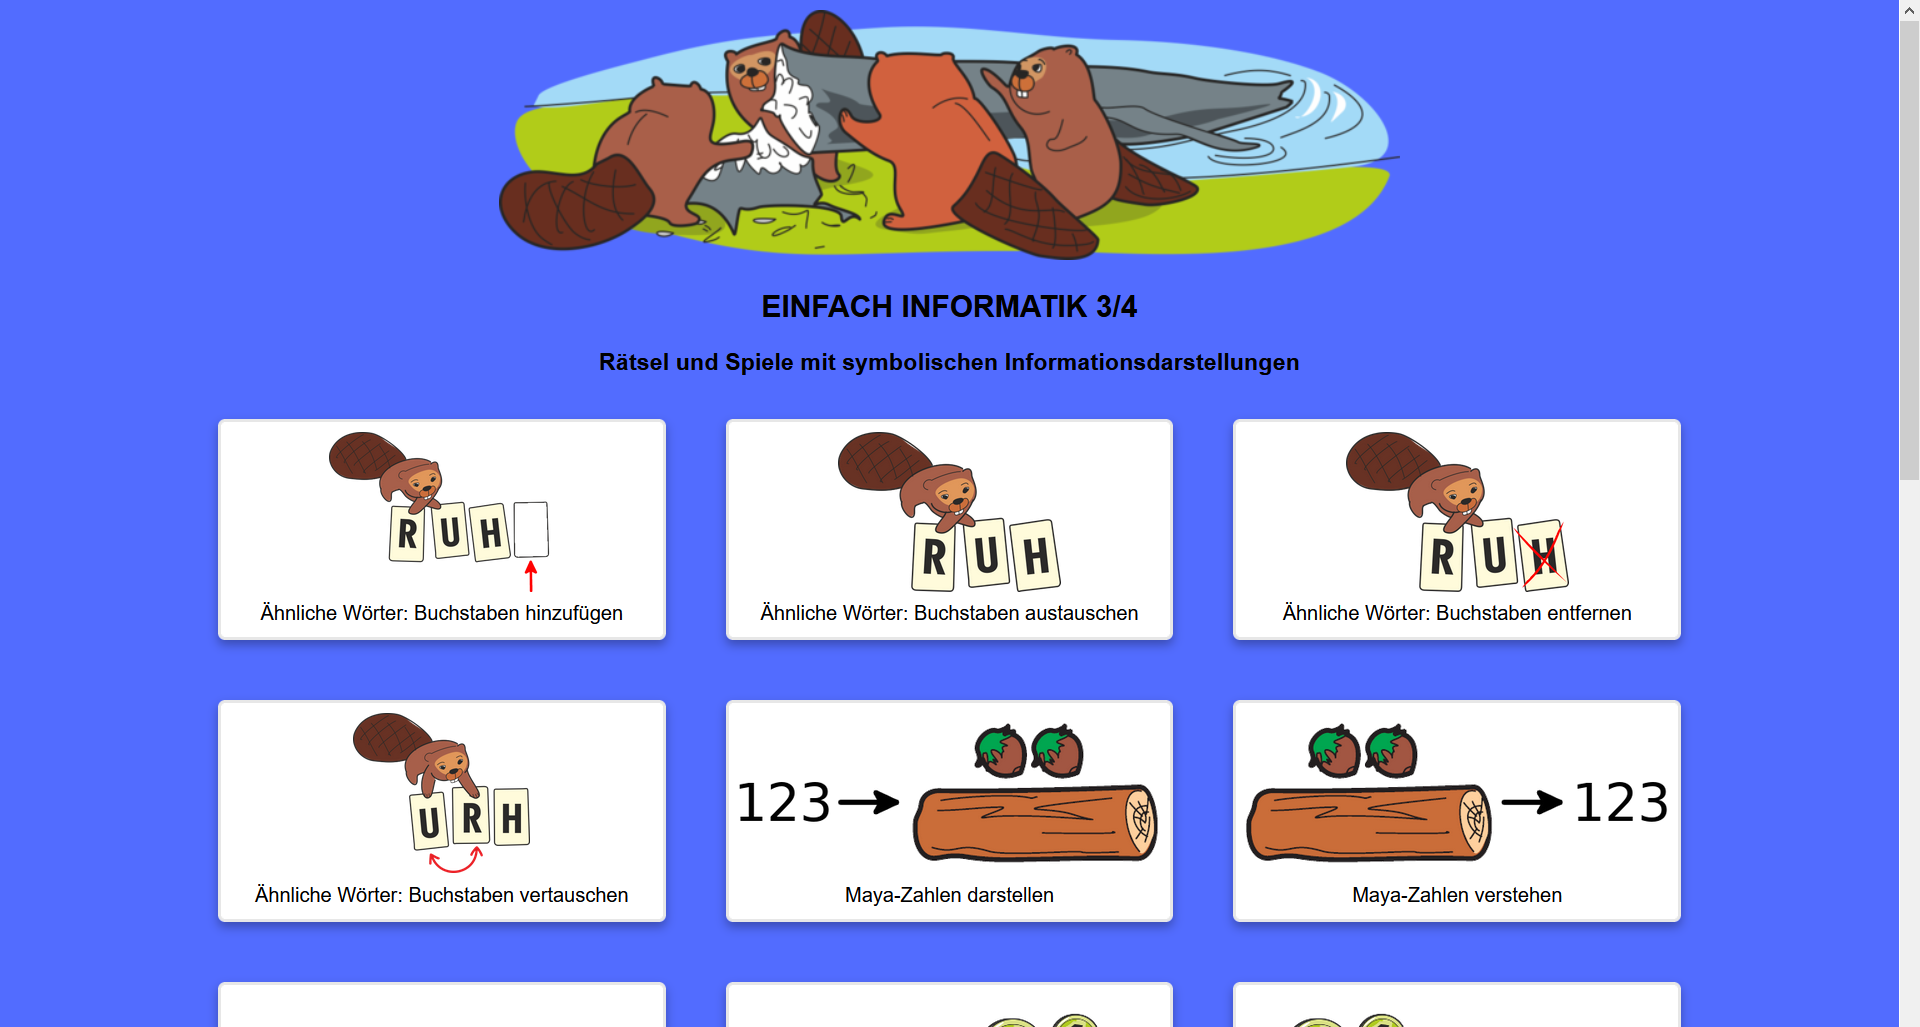
\includegraphics[width=1.0\columnwidth]{figures/P22.png}
    \caption{In-Game Snapshot of Option 2}
    \label{fig:P22} 
\end{figure}

\subsection{Decision and Justification}
The choice was made to build up a new environment according to option 2 in order to keep the freedom to program games without restrictions and to create a design that is appealing for third and fourth graders. Thereby, the interconnection to the already existing environment for "einfach Informatik 3/4" \cite{FBBT} is facilitated by this choice.

\section{Vue.js}
\label{section:vuejs}
The obvious choice to implement option 2 was to choose Vue.js as the main framework. Vue.js is a web framework developed several years ago by Evan You. It is built on top of JavaScript and features reactivity, which means that changes to the data of the application are directly applied and can immediately be seen by the user. Also, Vue.js features direct bi-directional communication between two components, given that they are in direct relation \cite{Vue}. The aforementioned features are major advantages when designing game-like tasks, as in this project. The main reason for this web framework was its simplicity in comparison to alternatives like Angular or React, and the fact that the existing environment for "einfach Informatik 3/4" also runs on Vue.js \cite{FBBT}.

Since the newest Vue.js version 3.0 was only a few months old when the project was launched, the choice was made to stick to the older version, namely version 2. This way, it was possible to ensure full library and web forum support. Version 2 has been established and proven itself as a solid framework for web applications \cite{Vue}.


\section{TypeScript}
\label{section:typescript}

For the choice of the underlying programming language, there were two options that are compatible with Vue.js: JavaScript and TypeScript. TypeScript was chosen since it is an extension to JavaScript and provides some additional functions. 

The latter is a scripting language that is dynamically typed. Informally, JavaScript helps to control how the website behaves. It can be used in browsers and runs on top of HTML and CSS, which are manipulated to enhance the user experience. JavaScript can receive, manipulate, and send data. JavaScript does not run on the server where all the information of a website is stored but on the user's computer, so it is run on client-side programming language. This leads to a shift of the workload and computational resources \cite{Javascript}. 

TypeScript extends JavaScript by providing type safety and concepts such as interfaces, method signatures, interfaces, enumerations and tuples. It provides a way to describe what type a variable has and helps to catch errors before the code is run. The type safety is assured during compilation from TypeScript to JavaScript \cite{Typescript}.

\section{HTML and CSS}
\label{subsection:html}
The choice of how to model the graphical interface was made along with the two previous choices. The common technologies for web development are HTML5 and CSS. HTML and CSS are core technologies that help building a website. They allow the developer to display program elements visually such that it can be seen by an end user. HTML is a descriptive language that enables the programmer to structure a website. CSS allows the software engineer to design and style a page in terms of colours, layouts, and fonts. JavaScript animates the content created by HTML and CSS files.

\section{Code Conventions}
As mentioned before, the design choices should support compatibility with other learning environments. Therefore, the technical structure of the learning environment is of fundamental importance.
The way code was written was adapted to some common, yet unofficial rules. The following list is a shortened citation of the documentation of the already existing learning framework for 'einfach Informatik 3/4' \cite{FBWT}. It represents some code conventions that help keeping a clean code structure and provide better readability. For each convention, code examples can be found in the Vue.js style guide \cite{VueStyleGuide}.

\begin{itemize}
    \item Always use \code{key} with \code{v-for} to maintain the internal component state.
    \item Avoid \code{v-if} with \code{v-for}
    \item Only the top-level \code{App} component and layout components should have global styles. All other components should always have scoped styles i.e. the style is only used within the component.
    \item Each component has its own file.
    \item Filenames are in PascalCase.
    \item Components without any content should be self-closing e.g \code{<Component />} instead of \code{<Component><Component/>}.
    \item Components name casing in templates is PascalCase.
    \item Properties name casing is camelCase.
    \item Elements with multiple attributes should span multiple lines, with one attribute on each line. [...]
    \item Element attribute values should be quoted.
    \item Directive shorthands are always used.
    \item Element attributes should be ordered consistently.
    \item Components should be ordered like \code{<templates>}, \code{<script>} and \code{<style>}.
    \item Element selectors should be avoided with \code{scoped}
    \item Properties and events should be used for parent-child communication.\cite{FBWT}
\end{itemize}

\section{Graphical Design}
The graphical design was chosen according to several criteria.
The fundamental criterion was that the design of the environment is intuitive and child-friendly. The young students should understand the functionality of the platform as good as possible. To facilitate this, the design and build-up of the webpages should be well-structured and there should not be too much content on a single page. The intuition should also be assisted by the choice of simple and modest colours. Last but not least, the learning environment should be similar to the already existing one for 'einfach Informatik 3/4' \cite{FBWT}, such that they could be merged later. 
\chapter{Architecture}
\label{chapter:architecture}

\section{Introduction}
\label{section:introduction}
In this chapter, the architecture of the learning environment will be regarded more closely. First of all, the central programming concept will be presented. Later, the general structure of the environment will be explained as well as the different parts.  Besides this, the goal is that an explanation for the design choices can be provided and a technical understanding for future additions to the program can be provided.

\section{Concept of Components}
\label{section:components}

In Vue.js, one can create program parts called components that can be reused in any part of the program \cite{Vue}. This can be highly useful, since many functions are used multiple times in a program, even with similar style and structure. Components can be used as a whole page (then called \nameref{section:views}) or as a part of a page or another component. For example, in every game a \nameref{subsection:buttonbar} for in-game functions is required. Instead of copying all the code for this function into every single game, one can create a component and then access it with a simple keyword. This improves not only the efficiency of the programmer, but also facilitates updates and keeps the code easy to read and understand. 

The project can be split up into components. The largest component is called App.vue. This component contains all the elements of the web application and will be rewritten and injected into the HTML file that then displays the website. App.vue contains all other components that are part of the learning environment. Each component contained in App.vue is called a child of the latter component, or even a grandchild, if it is nested within another component that is in App.vue.


\section{Layout}
\label{section:layout}
As presented in the previous section, the design concept of the learning environment requires the build-up and layout of any page of the program to be as simple and intuitive as possible. In order to cope with these requirements, the layout of the page contains of two main building blocks. The first block is the navigation bar on top of every page and the second is the routing container that displays the currently selected page. In the following, both integral parts of the platform are analysed more closely and their interconnection will be elaborated.


\subsection{Navigation Bar}
The navigation bar is placed in the top right corner of the page. For each page, it individually displays all the necessary functions that help to navigate or perform a special action. Here, one can find all buttons that are not directly involved with the task itself. All other buttons can be found in the game button bar. The navigation bar contains a function to return to the home screen, browse the about page, a print, full screen, and language switch function.

\subsubsection{Home Button}
The home button appears whenever the user is visiting another page than the home screen. This enables one to return to the main menu independent of which page has been loaded.


\begin{figure}[h]
    \centering
    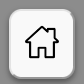
\includegraphics[width=0.2 \columnwidth]{figures/home.png}
    \caption{The Home Button} 
    \label{fig:next} 
\end{figure}

\subsubsection{Print Button}
The print button, represented by the printer icon, allows the user to print out a page. The page is formatted such that it can be printed in a better way. The program automatically renders all the relevant components in landscape mode and without the button menu and the navigation bar that are not needed on a printed page. Please note that on most computers, the print button does only print in landscape mode, as there is not enough space in portrait mode to print the whole page correctly. An example can be found in figure \ref{fig:printex}.

\begin{figure}[h]
    \centering
    
\includegraphics[width=0.2 \columnwidth]{figures/print.png}
    \caption{The Print Button} 
    \label{fig:next} 
\end{figure}

\begin{figure}[h]
    \centering
    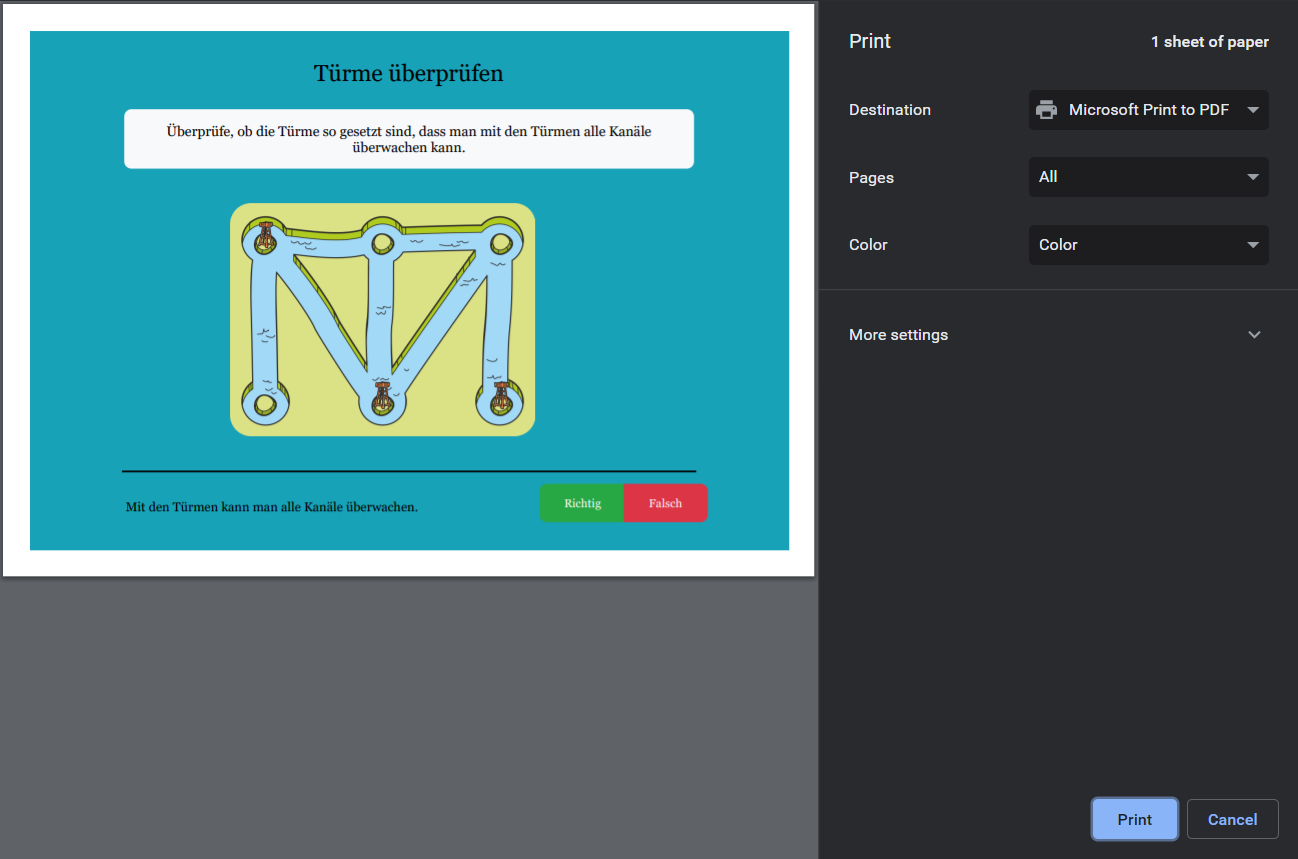
\includegraphics[width=1.0 \columnwidth]{figures/print_example.png}
    \caption{Example of a Print Window} 
    \label{fig:printex} 
\end{figure}

\subsubsection{Language Selector}
\label{subsection:language}
The language button contains the abbreviation of the language in which the environment runs momentarily. On click, the language is switched to the next available language. This button iterates through all available languages until it reaches the original language. This  is editable when one adds languages as an entry to the array 'languagePool' in the main app 'App.vue' together with a corresponding language file in the source folder in JSON format, that is named 'text\_[X].JSON', where [X] denotes a placeholder for the respective array entry of 'languagePool'. Every new language file must contain all elements and fields that the original German language file called 'text\_de.JSON' has. Otherwise, a correct functionality of the platform cannot be guaranteed.

\begin{figure}[h]
    \centering
    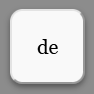
\includegraphics[width=0.15 \columnwidth]{figures/language.png}
    \caption{The Language Selector} 
    \label{fig:next} 
\end{figure}

\subsubsection{Information Button}
The information button is depicted by an encircled letter \textit{i}. It leads directly to the \nameref{subsection:about} page. This button can be found on the home screen and provides various information about the project and the learning environment.

\begin{figure}[h]
    \centering
    
\includegraphics[width=0.15 \columnwidth]{figures/about.png}
    \caption{The About Button} 
    \label{fig:next} 
\end{figure}

\subsubsection{Full Screen Button}
The button covered with a diagonal double arrow allows the user to switch from normal browser mode to full screen mode and vice versa. In full screen mode, the user experience is enhanced since all components find enough space to be properly displayed. Besides, there are no distractions when solving the tasks.

\begin{figure}[h]
    \centering
    
\includegraphics[width=0.15 \columnwidth]{figures/fullscreen.png}
    \caption{The Full Screen Button} 
    \label{fig:next} 
\end{figure}

\subsection{Routing Container}
The second main component of the page layout is the routing container. Depending on the current URL and choices made by the user, this component renders and displays different pages, in technical terms 'views'. Views correspond to different pages of the website. In the following section, views will be examined more closely. 

To enable routing to a new page, the programmer has to add the new page to a file called Views.js that is located in a folder that is called Views as well. There, the link, view and component of the new page can be specified, and the new link is automatically generated in the file index.ts that can be found in the folder called routing.

\section{Views}
\label{section:views}

As mentioned before, each page that is loaded consists of a full-page component called view and the navigation bar. Informally speaking, each so-called view corresponds to a page of the website.  Hence, there exists a view for the start page, the about page, for each game, et cetera. A view defines the build-up and layout of a page. It also specifies, which components are to be injected when rendering the page.

In the following, some particular views are presented. This will help to understand the general structure of the program.

\subsection{Home View}
The home page is the starting point whenever someone visits the website. It consists of an introductory section and a task-selector. The former gives a quick introduction to the online environment  (see figure \ref{fig:homescreen}). The latter presents the different task sets with all its levels. Each game is displayed in a box with description and a corresponding image.

\begin{figure}[H]
    \centering
    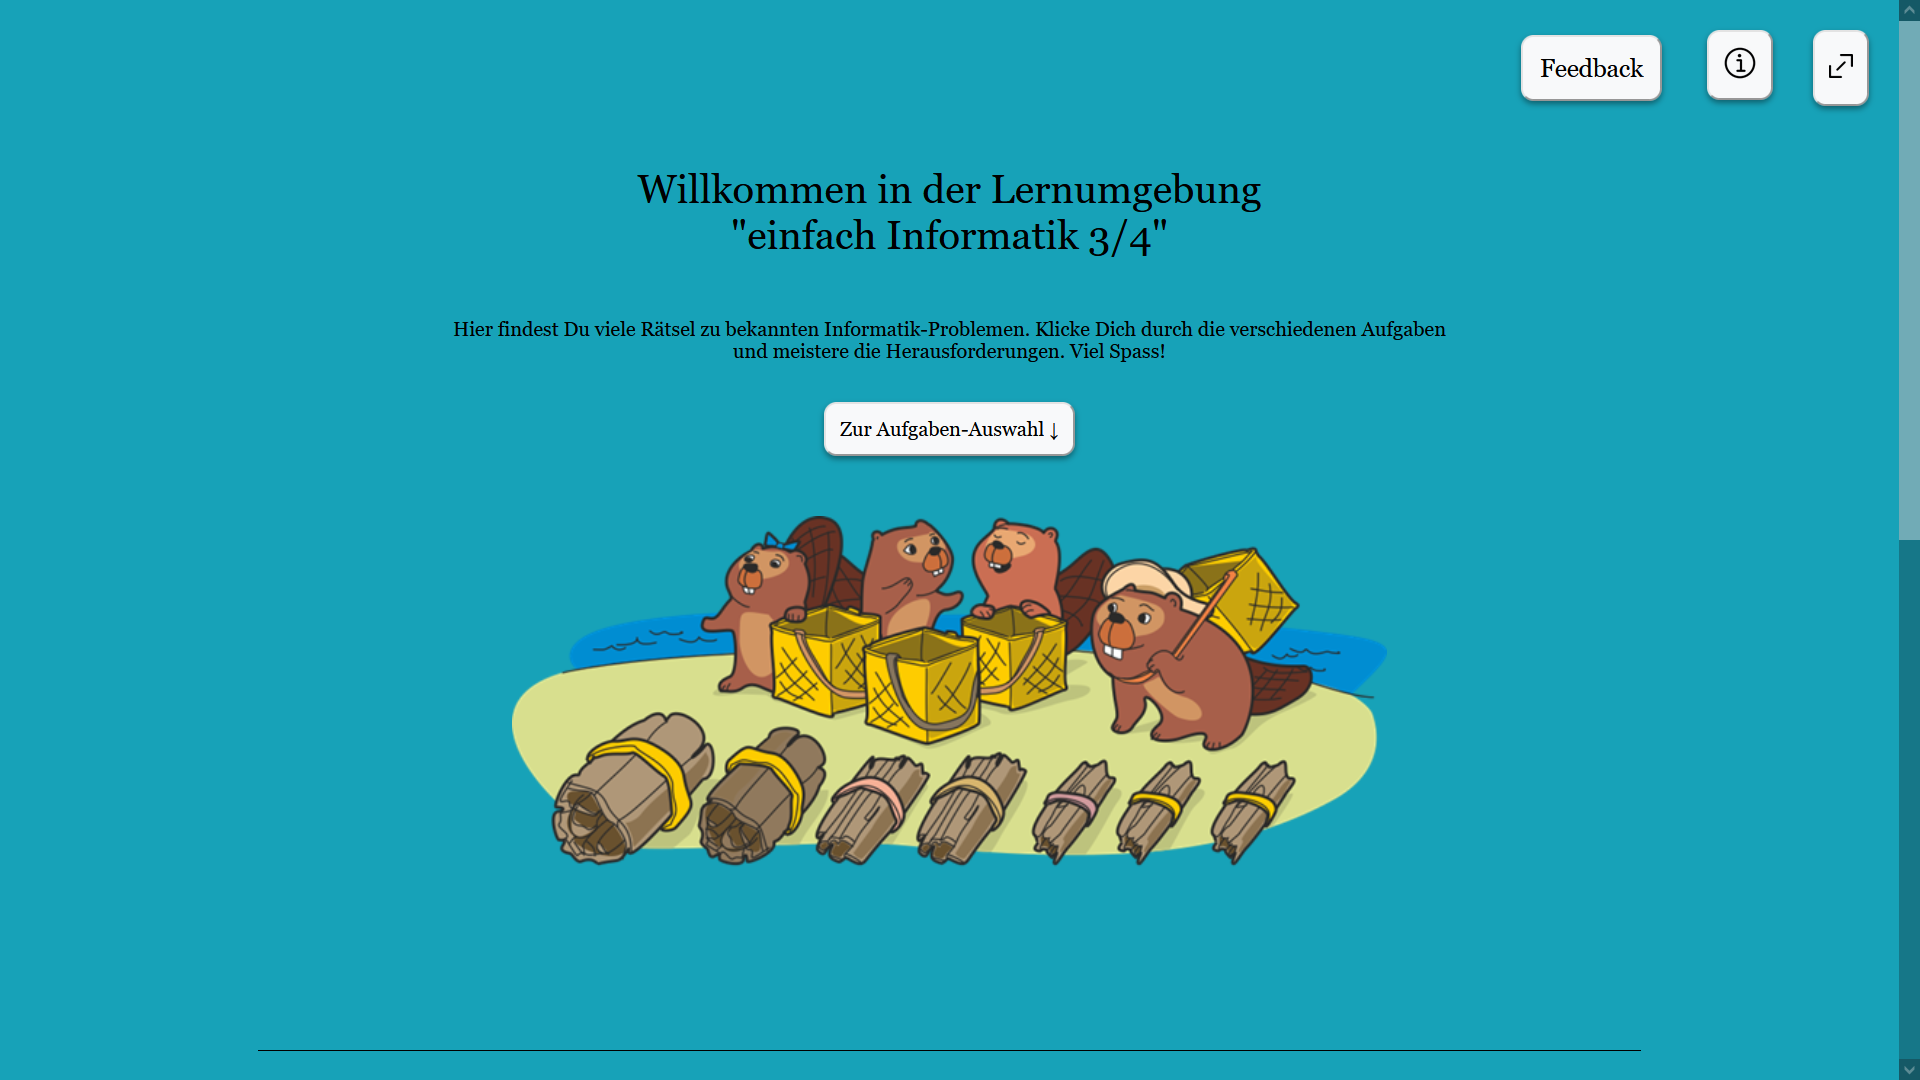
\includegraphics[width=1.0 \columnwidth]{figures/homescreen.png}
    \caption{The Home Screen} 
    \label{fig:homescreen} 
\end{figure}

\subsubsection{Task Selector}
The task selector gives an overview of all available tasks. For each game, there is a  box with the task title and a corresponding image (see figure \ref{fig:tasks}).

This container automatically lists all games that are part of the JSON file called text\_de.JSON or the file corresponding to the selected language. Any game that has been implemented and has a correct working link to access it can be added to this outline by adding it to the game section in the aforementioned JSON file.

\begin{figure}[H]
    \centering
    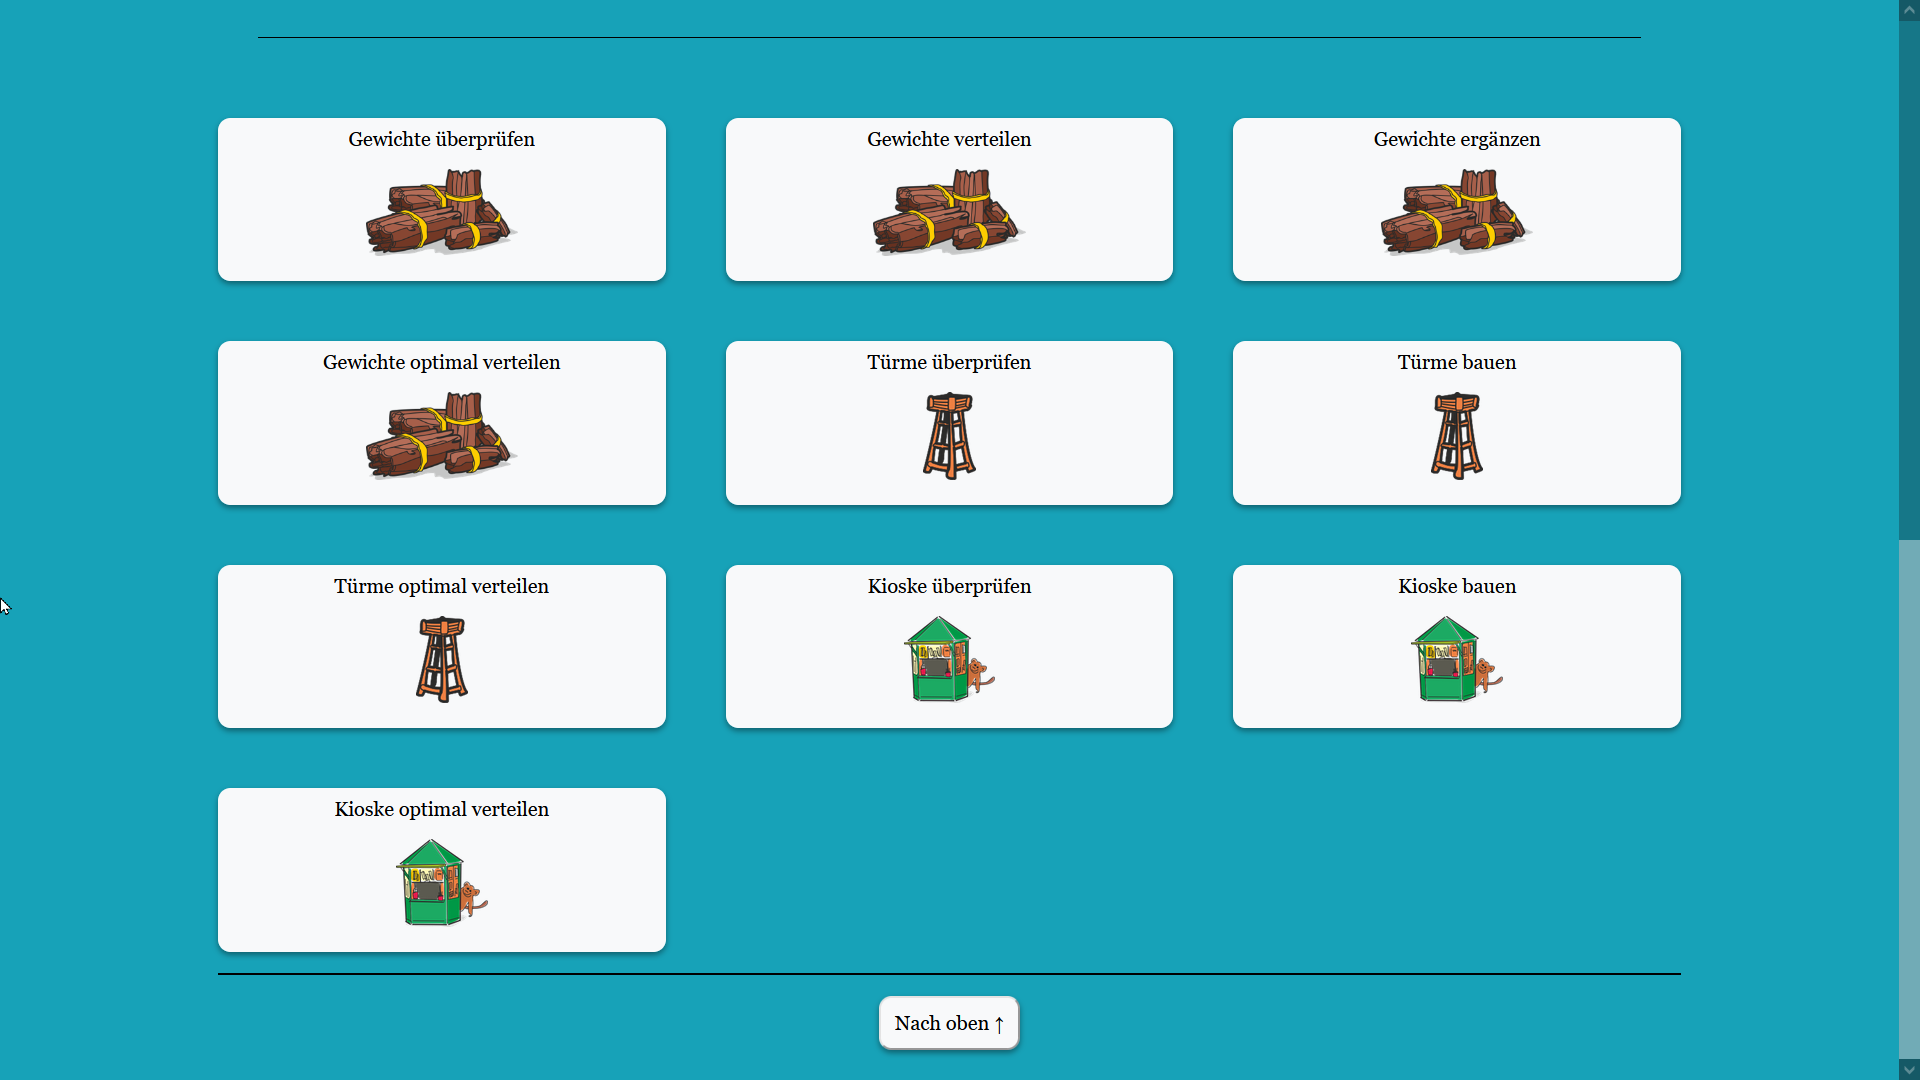
\includegraphics[width=1.0 \columnwidth]{figures/tasks.png}
    \caption{The Task Selector} 
    \label{fig:tasks} 
\end{figure}

\subsection{About View}
\label{subsection:about}
This view contains - like every other about page - all relevant information about the learning environment (see figure \ref{fig:aboutview}). Here, one can find the version, on which the platform is running. It can be useful to know what the newest features are and if the program has been updated recently. Further, information about the author and licences is provided.

\begin{figure}[H]
    \centering
    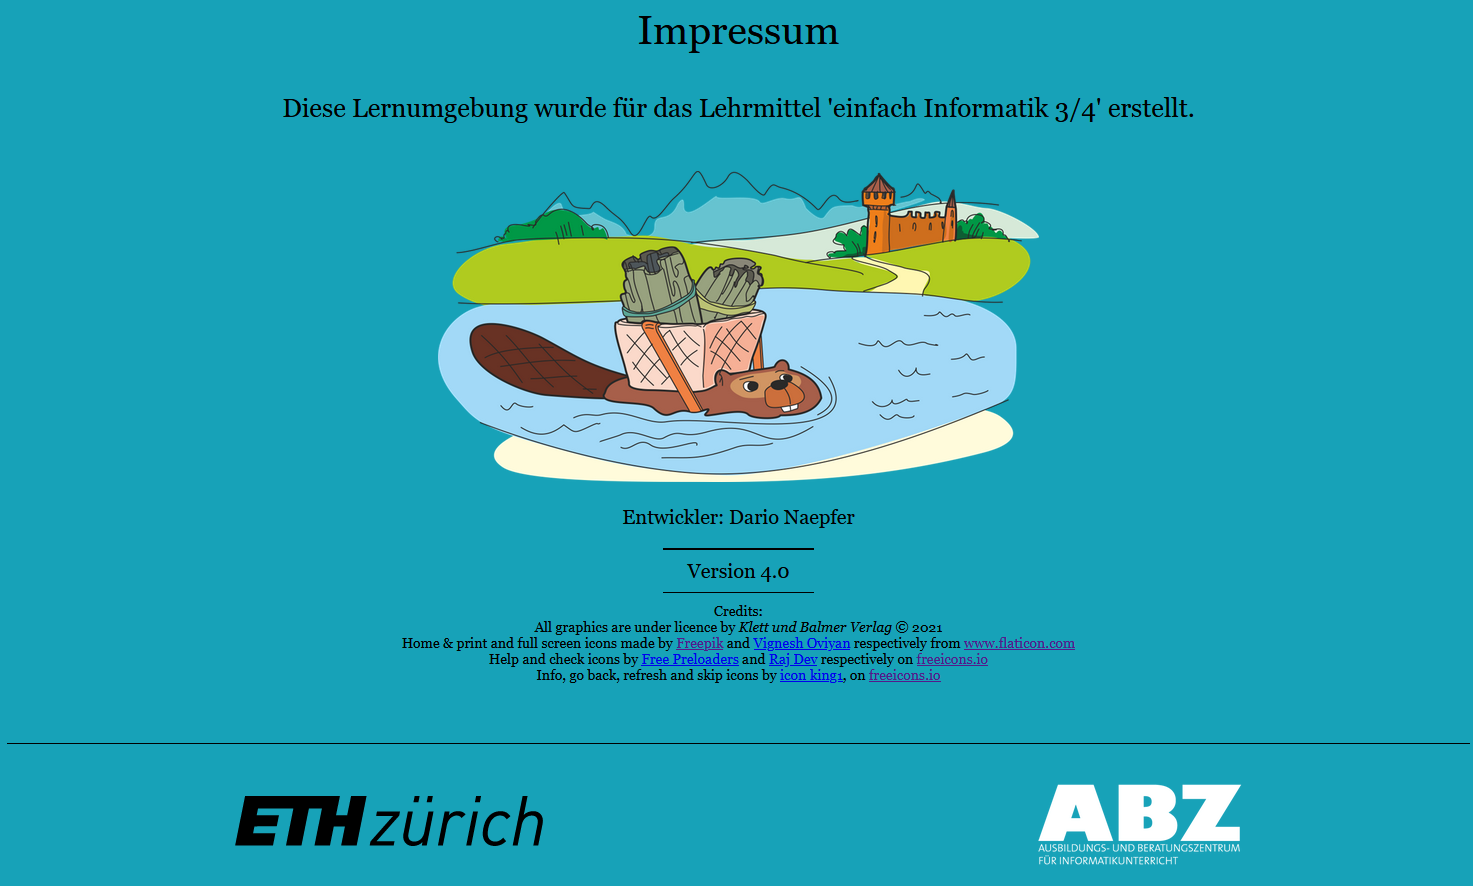
\includegraphics[width=1.0 \columnwidth]{figures/about_view.png}
    \caption{The About View} 
    \label{fig:aboutview} 
\end{figure}

\section{Game Component}
\label{section:game}

\subsection{Introduction}
The game component is the heart of the learning environment. The game component defines the general structure of the individual tasks. In this container, the game and all its features are displayed. On top of the page, there is a title referring to the actual task. The task is then introduced by an instruction sentence describing the exercise. This short introduction aims to give the user an intuition of how the task works. For more detailed explanations, one can open the instruction page for the task (see section on \nameref{subsubsection:tutorial}).

\subsection{Button Bar}
\label{subsection:buttonbar}
On the left-hand side of the game page, a button menu is displayed providing quick in-game functions. The buttons consist of symbols that give an intuition of the function they provide. When hovering over a button, the button floats to the right, and an additional description is displayed; otherwise, the text is hidden. In this way, the button menu is not too spacious and still clearly indicates its functions. There are four buttons in the following top-down order:

\subsubsection{Next Button}
The next button is represented by a right arrow. When clicked, either a new game is randomly generated or the game component is reloaded with a new map, depending on the current task. This button also resets all current game states such that a completely new task is initialized. 

\begin{figure}[H]
    \centering
    
\includegraphics[width=0.2 \columnwidth]{figures/next.png}
    \caption{The Next Button} 
    \label{fig:next} 
\end{figure}

\subsubsection{Reset Button}
The reset button is symbolized by a circular arrow. On click, a function is called that completely resets the current game state such that the current game can be played again from its initial position. Clicking this button does only affect the recent user inputs concerning the actual task.

\begin{figure}[H]
    \centering
    
\includegraphics[width=0.2 \columnwidth]{figures/restart.png}
    \caption{The Reset Button} 
    \label{fig:next} 
\end{figure}

\subsubsection{Verify Button}
The tick surrounded by a circle depicts the check button that can be called whenever an input should be verified. When the button is clicked, a pop-up window opens giving individual feedback on how well the task has been solved, including a beaver (see figure \ref{fig:beavers}). The user input is evaluated as either correct or incorrect. On a correct input, the modal window shows a celebrating beaver indicating that the task has been successfully completed. If this is not the case, a disappointed beaver is displayed coupled with a feedback or tip depending on the improvements that ought to be made. The user is advised to either first comply with the instructions or rethink the provided solutions.

\begin{figure}[H]
    \centering
    
\includegraphics[width=0.2 \columnwidth]{figures/check.png}
    \caption{The Verify Button} 
    \label{fig:next} 
\end{figure}

\begin{figure}[H]
    \centering
    
\includegraphics[width=0.7 \columnwidth]{figures/evaluation_result.png}
    \caption{The two beavers indicating the result correctness} 
    \label{fig:beavers}
\end{figure}

\subsubsection{Tutorial}
\label{subsubsection:tutorial}
The encircled question mark represents the tutorial button. By clicking it, one can find a more detailed description of the current task. The tutorial opens up in an overlay window that consists of a title, an extensive description as well as a tutorial video, individually created for each task or task set. An example is provided in the figure below.

\begin{figure}[H]
    \centering
    
\includegraphics[width=0.2 \columnwidth]{figures/tutorial.png}
    \caption{The Tutorial Button} 
    \label{fig:tutorial} 
\end{figure}

\begin{figure}[H]
    \centering
    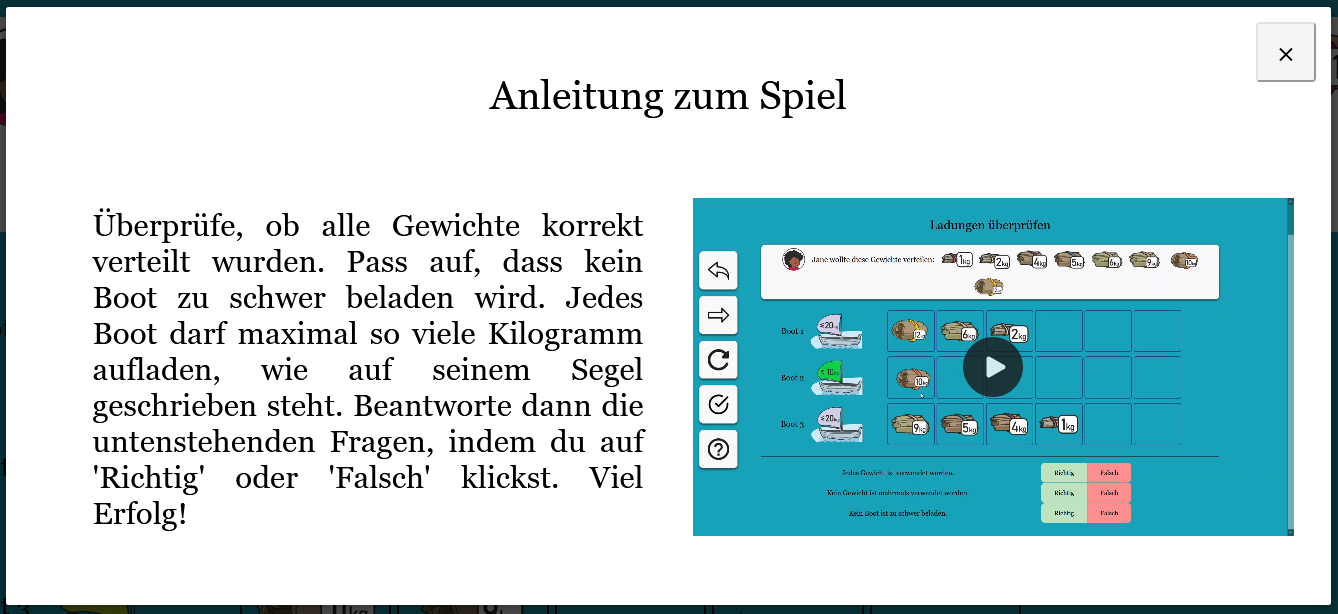
\includegraphics[width=1 \columnwidth]{figures/tutorial_example.png}
    \caption{Example of a Task Tutorial} 
    \label{fig:next} 
\end{figure}

\subsection{Difficulty Switch}
In one of the tasks, one can also find a difficulty switch in this section. On click, the difficulty is toggled between a lower difficulty level illustrated by a single standing beaver and a higher difficulty level depicted by two beavers. Whenever the button is clicked, the game is completely restarted and a new game instance is created.

\begin{figure}[H]
    \centering
    
\includegraphics[width=0.4 \columnwidth]{figures/levels.png}
    \caption{The Difficulty Switch} 
    \label{fig:levels} 
\end{figure}

\newpage
\subsection{Statement Check}
\label{subsection:statementcheck}
In each of the three task types, there is a difficulty level where suggested solutions for the task have to be reviewed by the user. Hence, a reusable component was created for this purpose. It can be integrated in each of the task templates. This component automatically generates a statement including a true/false button for each string that is passed as an argument. True and false can be toggled by clicking on the statement itself or on the corresponding button. The parameter called statements is an array with tuples consisting of a number and a statement. The array can contain any number of tuples and will create a proposition for each string.

\begin{figure}[H]
    \centering
    
\includegraphics[width=0.3 \columnwidth]{figures/tf-buttons.png}
    \caption{The Statement Check Buttons} 
    \label{fig:statement} 
\end{figure}

\chapter{Task Concept}
\label{chapter:concept}

\section{Introduction}
\label{section:introduction}
The main objective of information technology is to automatize the search for solutions if tasks are assigned. Here, this concept will be applied to algorithmic problems. The latter term describes a collection of tasks of high similarity, also called problem instances in this thesis. Due to high similarity, such task collections can be solved with a specific individual algorithm. An algorithm is a universal method consisting of precise rules describing how to solve any problem instance of the corresponding problem set.

In this chapter, the general idea behind the task sets will be presented. This includes the didactic idea underneath the task levels, as well the design of the different variations in each task set.

\section{Difficulty Levels}
\label{section:levels}

The main goal that underlies the learning environment is to equip students to be able to solve problems on their own. According to Bloom's Taxonomy, there are different levels of complexity depending on the cognitive dimensions of a task. The levels of each task set are designed accordingly: Starting with simple challenges called classification tasks, the tasks are designed such that the difficulty of the assignments improves gradually. In this way, they are introduced step by step into the algorithmic concepts that should be acquired. Active learning and self-improvement is promoted. The students should learn to think in a way that enables them to approach new challenges and assignments with sophisticated steps and to solve them.

The tasks are designed such that the different levels of a task set look very similar. This creates a recognition value, meaning that the user has already been familiarized with the problem and thus knows the general concept of the task. 

With the possibility of multiple permissible solutions for most problem instances, the student's creativity is required and promoted. The students learn to solve similar problems with yet different solutions.

With random distributions that are included in a majority of tasks, the students are required to solve the task on their own since there is no solution or hint from an external source like the neighbour's screen.


\section{Level 1 - Verify Solutions}
\label{section:verify}
The first difficulty level tests the student's capability to interpret a given problem set together with a provided proposition for a solution to the problem. The proposition then has to be categorized as either a correct or incorrect proposition. A proposition is permissible if and only if it fully complies to the task specifications. The tasks are modelled as decision problems where the user has to answer at least one question regarding the correctness of the proposition. The student is required to interpret the proposition of the problem instance correctly, fully understand the criteria, and then evaluate the given solution proposition accordingly. Furthermore, in some cases, the students learn to justify why a specific problem instance is or is not permissible.

\section{Level 2 - Find Solutions}
\label{section:find}
At this difficulty level, the user is confronted with a task for which he or she has to find a permissible solution on his or her own. The learning objective is to take the matter into one's hand and actively find ways to deal with a new challenge. This is more difficult than just verifying solutions, since the student's creativity to come up with an own solution is required. The only condition a solution must fulfil is that the proposed solution has to be valid, the quality of the solution is not taken into consideration on this level. All solutions are considered of equal value.
For one exercise type, there is an advanced version of this level: The  \nameref{chapter:weights} exercise has another level that instructs the user to find a solution by him- or herself as well. In this case, however, the computer has already taken several steps towards a permissible solution proposition, so the amount of permissible solutions decreases a lot. This makes the exercise more difficult to solve than the regular level 2 exercise.

\newpage
\section{Level 3 - Optimize Solutions}
\label{section:optimize}
The highest difficulty level requires from the user to compare different solution propositions according to given criteria. The user has to compare the quality of these propositions and then decide for the optimal solution. Here, it is imperative that the possible solutions are strictly limited. The variety of the solutions must be small enough that the student is able to list all the different solutions and can then decide which one is the optimal proposition.
\chapter{Weights}
\label{chapter:weights}

\section{Introduction}
\label{section:introduction}
The first task set is concerned with the transport of goods and of key importance in information technology and finds various application fields. Associated to this task is a well-known problem in the field called 'rucksack problem'. The tasks modelled here are simplified and do not require the solution to fulfil as many conditions as in the rucksack problem. 

In this task set, different weights, labelled with 1 to 12 kilograms (see figure \ref{fig:weights}), are available and can be distributed among boats of different capacities (see figure \ref{fig:boats}). Throughout the levels, the user has to check and distribute the weights. The condition for a solution to be valid is that all weights of the initial weight set are used and that no boat is overloaded.


\begin{figure}[H]
    \centering
    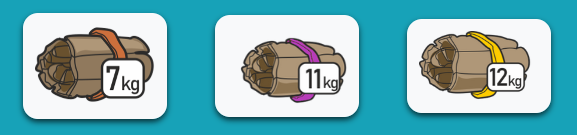
\includegraphics[width=0.6 \columnwidth]{figures/weights.png}
    \caption{Weights of Different Sizes} 
    \label{fig:weights} 
\end{figure}

\begin{figure}[H]
    \centering
    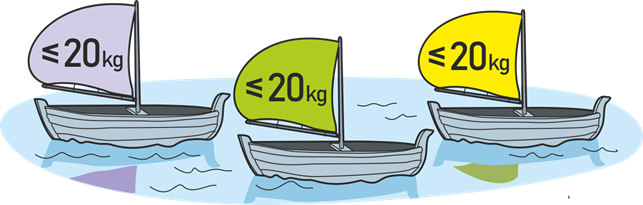
\includegraphics[width=0.6 \columnwidth]{figures/boats.png}
    \caption{Boats with Weight Capacities} 
    \label{fig:boats} 
\end{figure}

\section{Levels and Goals}
\label{section:assignment}

The goal of this exercise set is to train the competence to plan and conduct transports of a given quantity while minimizing the effort and resources assigned to it. 

On the first level, the students are required to observe all the given weights closely. There may be weights that have not been distributed in spite of being on the distribution list. Also, some weights may show up twice or even a weight that is not on the original list might have been added. The students learn to double-check the solution proposition and have to answer several questions accordingly.

The second level then assigns a distribution task to the students. They have to place all the given weights onto the different boats, such that no boat is overloaded. The user has to find a permissible solution by him- or herself, and thus is required to find strategies to balance the different weights between the different boats

On the third level, the task is to complete a solution proposition. Additionally to the initial position of the level 2 task, the algorithm has already placed a few weights on boats. Since some steps are fixed, the amount of permissible solutions often decreases. The user then has to find a valid solution, given this starting position.

On the fourth level, the user has to minimize the number of boats, on which the weights are distributed. So, besides finding a valid solution such that all weights are in use and no boat is overloaded, the assignment is to find the best solution. The user is thus encouraged to consider and compare multiple solutions and evaluate them according to the given criterion.


\section{Implementation}
\label{section:implementation}
The implementation of the task levels are based on two different templates. The first template is called WeightCheck.vue and fully defines the design and functionality of the first level, where the user has to check if the boats are correctly loaded with weights. The second template covers the remaining three difficulty levels, named Weights.vue. The different templates define the main structure of the tasks. In WeightCheck.vue, there is additionally a \nameref{subsection:statementcheck} that is rendered below the component that contains the boats.
Each level has its own corresponding view, called CheckWeights.vue, DistributeWeights.vue, AddWeights.vue, and OptimizeWeights.vue, ordered increasingly. This means that each task level has its own page, where the details of the task are specified. The functionality and the algorithm behind the tasks are stored in the templates, however, as mentioned before.

Before the task can be solved, all elements of the exercise have to be initialized. In this case, the non-deterministic random algorithm has to be run. The weights are randomly chosen from a weight set containing weights from 1 to 12 kilograms for each level and each problem instance. This task is accomplished by first choosing a random number for the boat capacity among all available boat sizes:

%TC:ignore
\begin{lstlisting}[language=TypeScript,caption={},label={lst:chooseBoatSize}]
ship1 = Math.floor(1 + Math.random() * 3) * 10;
\end{lstlisting}
%TC:endignore

The previous steps are executed on every level except for the first difficulty degree of the task. When all boat sizes are determined, the new maximal weight sum (here: newWeightSum) is known and the random weight set can be generated. This is done by setting a range of accepted total weight sums and then adding weights to the set as long as the chosen weight sum (here: chosenWeightSum) is not yet in the range of accepted weights.

%TC:ignore
\begin{lstlisting}[language=TypeScript,caption={},label={lst:chooseWeights}]
chooseWeights() {
    while (chosenWeightSum + sentinel <= newWeightSum) {
        randomWeight = Math.floor(1 + Math.random() * maxWeightSize);
        if (!chosenWeights.has(randomWeight)) {
          chosenWeights.add(randomWeight);
        }
    }
}
\end{lstlisting}
%TC:endignore

Next, the weights are distributed among the boats. This step is necessary to ensure that it is possible to find a solution. There are problem instances with weight selections that have no solutions. These are avoided since the weight selection is always double-checked such that there exists at least one permissible way to distribute the given weights for every task that is presented to the user.

%TC:ignore
\begin{lstlisting}[language=TypeScript,caption={},label={lst:distributeWeights}]
distributeWeights() {
    // iterate through all chosen weights and distribute them
    for (let i = 0; i < weights.length; i += 1) {
        for (let j = 0; j < boatCapacities.length; j += 1) {
            if (weights[i] <= boatCapacities[j] - actualBoatLoad[j]) {
              addWeight(weights[i], j); //add weight i to boat j
              break;
            }
        }
    }
}
\end{lstlisting}
%TC:endignore

Depending on the level, the weights are displayed differently, and different solution checks are run over the user input. The first level requires from the student to check a given solution. In this case, the weights that have been distributed are placed in all slots corresponding to the boats and then made visible. Also, all weight movement functions are disabled such that only the true or false buttons can be selected. The user's answers to the questions then simply are compared to the generated solution. 

The level 2 task does not display the correct distribution and instead displays an item selection zone below the boats such that the user can manually distribute the weights among the boats. Additionally for the level 3 initialization, some weights are picked and already placed on specific ships. These weights are added to a list called fixedWeights that can not be modified by the user. At both levels, the user weights are added up and compared to the boat capacities. Also, it is checked if all weights are used. If this is the case and all requirements are met, the proposition is accepted.

Level 4 runs the same checks as in level 2 and 3, but additionally checks whether the correct boats are used that are included in the optimal solution. The boats of this solution are stored in boatUsedOpt and then compared to the boats that are used by the student's solution, stored in the array boatUsed.

%TC:ignore
\begin{lstlisting}[language=TypeScript,caption={},label={lst:isOptimalSolution}]
isOptimalSolution(level:number):boolean {
    for (let i = 0; i < boatUsed.length; i += 1) {
      if (boatUsed[i] !== boatUsedOpt[i]) {
        return false;
      }
    }
    return true;
  }
\end{lstlisting}
%TC:endignore
\chapter{Towers}
\label{chapter:towers}

\section{Introduction}
\label{section:introduction}
This task set is about building towers on islands and models an important graph problem in the field of information technology. The algorithmic problem lying beneath this task is called Vertex Cover. For a given graph with vertices and edges, the algorithm tries to find a minimal set of vertices such that every edge of the given graph has an incident vertex that is part of the selection.

In this task set, a tower (see figure \ref{fig:tower}) can be selected and built on islands. There are different maps containing a network of water channels and islands (see figure \ref{fig:map}).
Throughout the levels, the user has to check and distribute towers. The challenge is to place towers in a way that all channels of the map can be observed. A channel can be observed if and only if it has a tower at the end of it or at the next intersection with another channel.

\begin{figure}[H]
    \centering
    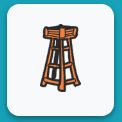
\includegraphics[width=0.2 \columnwidth]{figures/tower.png}
    \caption{Tower} 
    \label{fig:tower} 
\end{figure}

\begin{figure}[H]
    \centering
    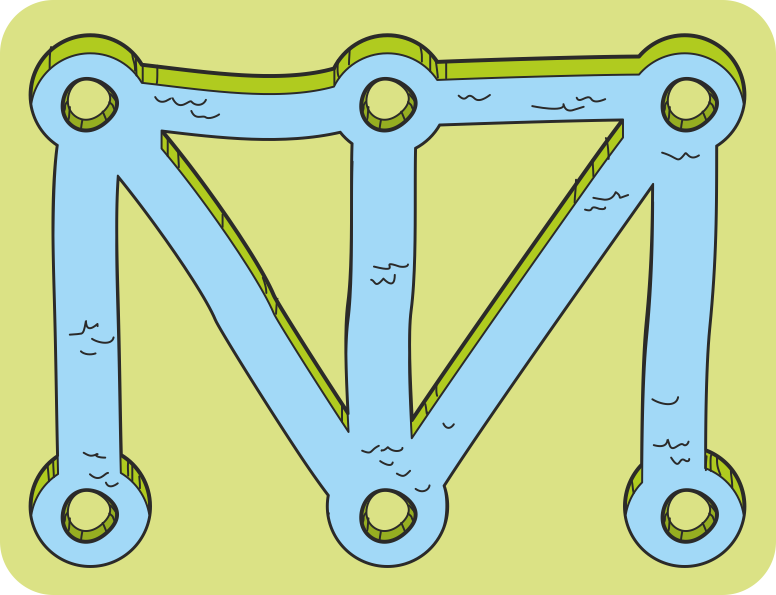
\includegraphics[width=1.0 \columnwidth]{figures/map_example.png}
    \caption{Example of a Map} 
    \label{fig:map} 
\end{figure}

\section{Levels and Goals}
\label{section:assignment}

The goal of this exercise set is to train the student's capability to find strategies to cover a graph with towers while minimizing the resources needed to do so. The users are encouraged to reflect on different positions where towers could be placed and how useful a particular drop zone is. 

On the first level, the students are required to check the placed towers whether they fulfil the condition that all channels can be observed. Often, there are channels that seem to be observed but are not since there is no adjacent tower.  

The second level then assigns a construction task to the students. They have to place a given number of towers onto the islands, such that all channels can be observed. For each map, the number of towers is set individually such that the task can be solved. Also, the number is kept small enough to prevent the user from placing a tower on every single island, which would be a trivial solution. The user has to find a permissible solution by him- or herself, and has to find ways to cover all the channels by trying out different approaches.

On the third level, the task is to find an optimal solution. The number of towers for an optimal solution is not explicitly mentioned, and thus one is required to find strategies to cover as many channels as possible with a single tower. The user is encouraged to consider and compare multiple solutions and evaluate them according to the given criterion.


\section{Implementation}
\label{section:implementation}
The implementation of the task levels is based on a game template and on a map template. The game template is called Towers.vue and defines the main structure and design. It also specifies the meta functionality like game generation, restart, and evaluation. The map template called TowersTemplate.vue then specifies the particular functions for a map that is then dynamically injected into the game template. In Towers.vue, there is additionally a \nameref{subsection:statementcheck} that is rendered below the component that contains the maps.

Each map has an underlying graph that is modelled according to the graph drawn on the map. This graph is modelled as an adjacency list and is based on a graph class providing all needed graph operations. The graph class can represent any directed or undirected graph and modify it by adding or removing edges and vertices.

%TC:ignore
\begin{lstlisting}[language=TypeScript,caption={},label={lst:graphClass}]
 class Graph {
  numberOfVertices;

  adjList;

  visitedNodes = new Set();

  queue = [0];

  constructor(vertices:number) {
    this.numberOfVertices = vertices;
    this.adjList = new Map();
  }
\end{lstlisting}
%TC:endignore

The testing is run over every solution proposition, independent if it was created by the computer or the user. The test checks if the proposition complies with all the regulations and consists of an algorithm that checks if the chosen vertex set forms a vertex cover. As a first step, all chosen vertices (contained in the array called arr) of the underlying graph are removed, including all incident edges (see code below). If the solution is correct, the towers cover all channels. When every vertex with a tower is removed, along with all edges symbolizing the channels, no edge or channel remains in the modified graph. The verification algorithm can be seen below in a simplified version:

\newpage
%TC:ignore
\begin{lstlisting}[language=TypeScript,caption={},label={lst:isVertexCover}]
  isVertexCover(arr:unknown[]):boolean {
    for (let i = 0; i < arr.length; i += 1) {
      removeVertex(Number(arr[i]));
    }

    const solution = isEmptyGraph();
    return solution;
  }
\end{lstlisting}
%TC:endignore

In a second step, the modified graph is tested on remaining edges. If the graph contains no edges, the solution is marked to be correct and permissible. 

%TC:ignore
\begin{lstlisting}[language=TypeScript,caption={},label={lst:isEmptyGraph}]
 isEmptyGraph():boolean {
    let empty = true;
    const getKeys = adjList.keys();
    for (const i of getKeys) {
      if (adjList.get(i).size > 0) {
        empty = false;
      }
    }
    return empty;
  }
\end{lstlisting}
%TC:endignore

The correctness of the level 1 proposition is immediately verified by the vertex cover algorithm when a random set is generated. Whenever the verify button is clicked, all the program does is comparing the user input to the result of the aforementioned algorithm.

The second level is reviewed by the verification algorithm as soon as the user has finished an own proposition and validates it. A solution is permissible if and only if the algorithm outputs true. 

Level 3 corresponds to the optimization task. Therefore, not only the regular checks as in level 2 are run, but also the optimality check is executed, which simply compares the number of used towers to the number of towers used in the optimal solution. Whenever both checks are evaluated positively, the result is emitted and marked as true.
\chapter{Kiosks}
\label{chapter:kiosks}

\section{Introduction}
\label{section:introduction}
This task set is concerned with building kiosks in villages and models another central graph problem in information technology. The algorithmic problem lying beneath this task is called Dominating Set Problem. For a given graph with vertices and edges, the algorithm tries to find a minimal set of vertices such that every vertex of the given graph has either the vertex itself or an adjacent vertex that is part of the selection.

In this task set, a kiosk (see figure \ref{fig:kiosk}) can be selected and then be built on a point in the graph. There are different maps containing a village network with points and interconnections (see figure \ref{fig:kioskExample}).
Throughout the levels, the user has to check given kiosk distributions and find own solutions. The challenge is to place kiosks in a way that all points of the map representing villages have close access to a kiosk. A village has close access to a kiosk if and only if it has a kiosk itself, or there is a neighbouring village with a kiosk.

\begin{figure}[H]
    \centering
    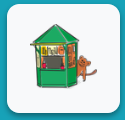
\includegraphics[width=0.2 \columnwidth]{figures/kiosk.png}
    \caption{The Kiosk} 
    \label{fig:kiosk} 
\end{figure}

\begin{figure}[H]
    \centering
    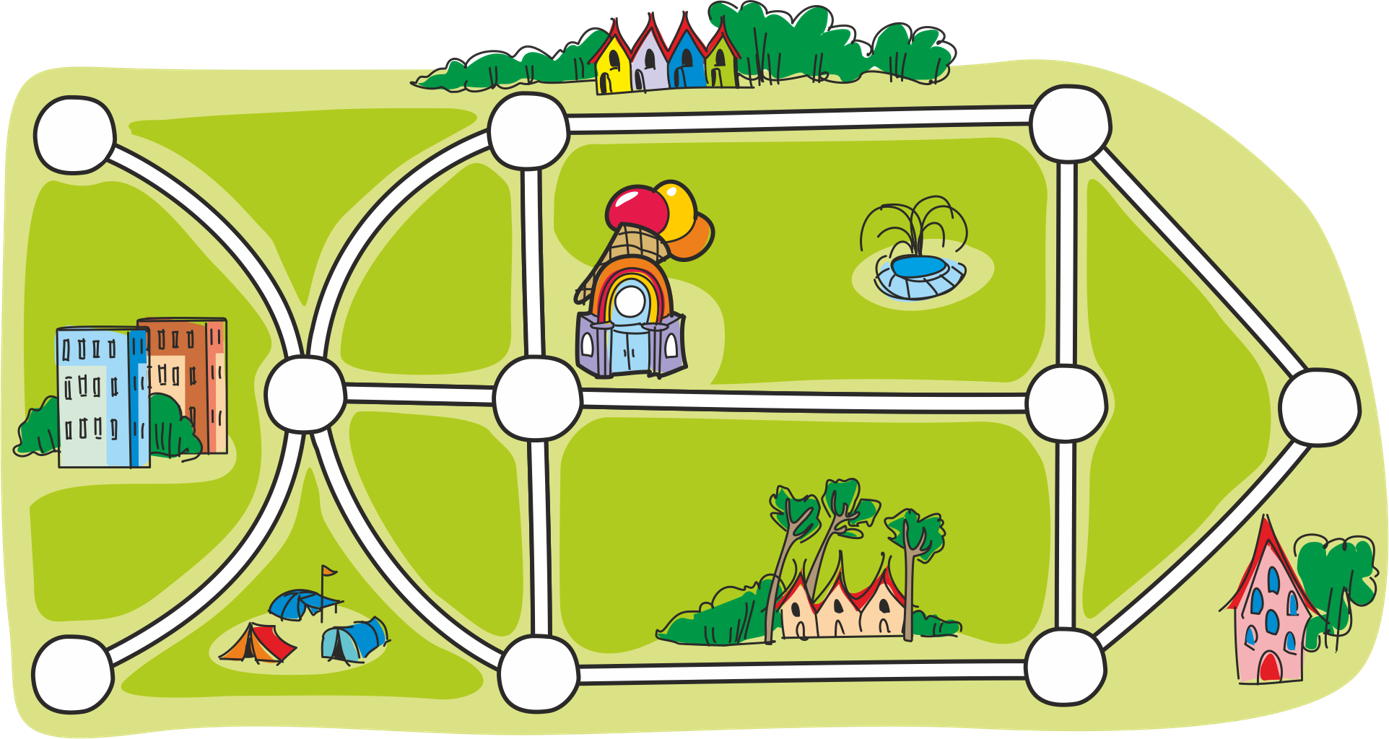
\includegraphics[width=1.0 \columnwidth]{figures/kiosk_example.png}
    \caption{Example of a Map} 
    \label{fig:kioskExample} 
\end{figure}


\section{Levels and Goals}
\label{section:assignment}

Similar to the previously discussed \nameref{chapter:towers}, the goal of this exercise is that the student finds strategies to cover a graph with as few kiosks as possible. The users are encouraged to reflect on different points in the graph where kiosks could be placed and how useful a particular place is (that is, how many villages it provides access to). 

The levels correspond to the structure of the towers exercise: On the first level, the students are required to check if the placed kiosks build a dominating set. Often, there are more villages covered with a single kiosk than the user would intuitively expect.

On the second level, the students have to build kiosks in villages, such that all villages have a kiosk close by. Again, the number of kiosks is set for each map individually. Also, the number is small enough such that kiosks cannot be placed on every single point.

On the third level, the task is to find an optimal solution. The number of kiosks for an optimal solution is not indicated.


\section{Implementation}
\label{section:implementation}
Similarly to the towers exercise, the implementation of the task levels is also based on a game template and on a map template. The game template is called Kiosks.vue and defines the main structure, design, and meta functionality. The map template called KiosksTemplate.vue then specifies the particular functions for a map that is then dynamically injected into the game template. Also, the \nameref{subsection:statementcheck} is located in Kiosks.vue.

Just as in the towers exercise, each map has an underlying graph that is modelled according to the graph drawn on the map. The graph is represented by the same graph class.

One of the main differences to the towers task set is the algorithm to test the correctness of a solution. The testing is run over every solution proposition, independent if it was created by the computer or the user. The test checks if the proposition complies with all the regulations and consists of an algorithm that checks - in contrast to the towers exercise - if the chosen vertex set forms a dominating set. As a first step, all chosen vertices (contained in the array called arr) of the underlying graph are added to a set called coveredVertices (see code below). Additionally, all neighbours of the vertex are added to the set when a vertex is checked and added to the set. If the solution is correct, the set contains every vertex of the graph after the algorithm has terminated. The verification algorithm can be seen below in a simplified version:

%TC:ignore
\begin{lstlisting}[language=TypeScript,caption={},label={lst:isDominatingSet}]
  isDominatingSet(arr:unknown[]):boolean {
    const coveredVertices = new Set();
    for (let i = 0; i < arr.length; i += 1) {
      for (const j of adjList.get(arr[i])) {
        coveredVertices.add(j);
      }
      coveredVertices.add(arr[i]);
    }

    // if every vertex has a marked neighbor, the set size corresponds to the total number of vertices
    const solution = (coveredVertices.size === numberOfVertices); // assigns a boolean value
    return solution;
  }
\end{lstlisting}
%TC:endignore

The correctness of the user input is verified just as described in the chapter on \nameref{chapter:towers}: The correctness of the level 1 proposition is immediately verified by the dominating set algorithm when a random set is generated. Whenever the verify button is clicked, all the program does is comparing the user input to the result of the aforementioned algorithm.

The second level is checked as soon as the user has finished an own proposition. A solution is permissible if and only if the user has chosen a dominating set.

In the optimization task, not only the implemented dominating set check is run, as in level 2, but the proposition is also tested if it is optimal. To do so, the algorithm simply compares the number of used kiosks to the number of kiosks used in the optimal solution. Whenever both checks are evaluated positively, the result is emitted and said to be true.
\chapter{Live Testing}
\label{chapter:testing}

\section{Introduction}
\label{section:introduction}
Towards the end of the implementation of the environment, the project was deployed on a test website and then tested in various schools and grades to ensure full functionality. In this way, feedback for minor adaptions and improvements was gathered, the testing gave an impression of the intermediate result. The testing was designed and arranged that students from a wide range in terms of origin, background, and academic performance were associated with the learning environment, such that authentic and representative feedback could be guaranteed. In the following, the test procedure will be thoroughly examined and explained before the results of the live testing feedback will be presented.

\section{Test Extent}
\label{section:procedure}

\subsection{Test Locations and Grades}
The testing phase was carried out in various schools in different regions of Switzerland. In Zurich, a majority of teachers of the elementary school Entlisberg agreed to participate in the test project. In total, in this school two fourth grades, a third grade and an extra class of specially talented pupil from second to eight grade completed the testing procedure (see figure \ref{fig:testing}). Besides, several groups of specially talented students of both third and fourth grade in the private school Cantaleum Zürich completed the test. A few teachers of other classes from various places also agreed to conduct the live testing by themselves and then provided feedback. In total, over a hundred people tested the platform. The feedback was collected, examined and evaluated in order to improve the learning environment. 

\begin{figure}[H]
    \centering
    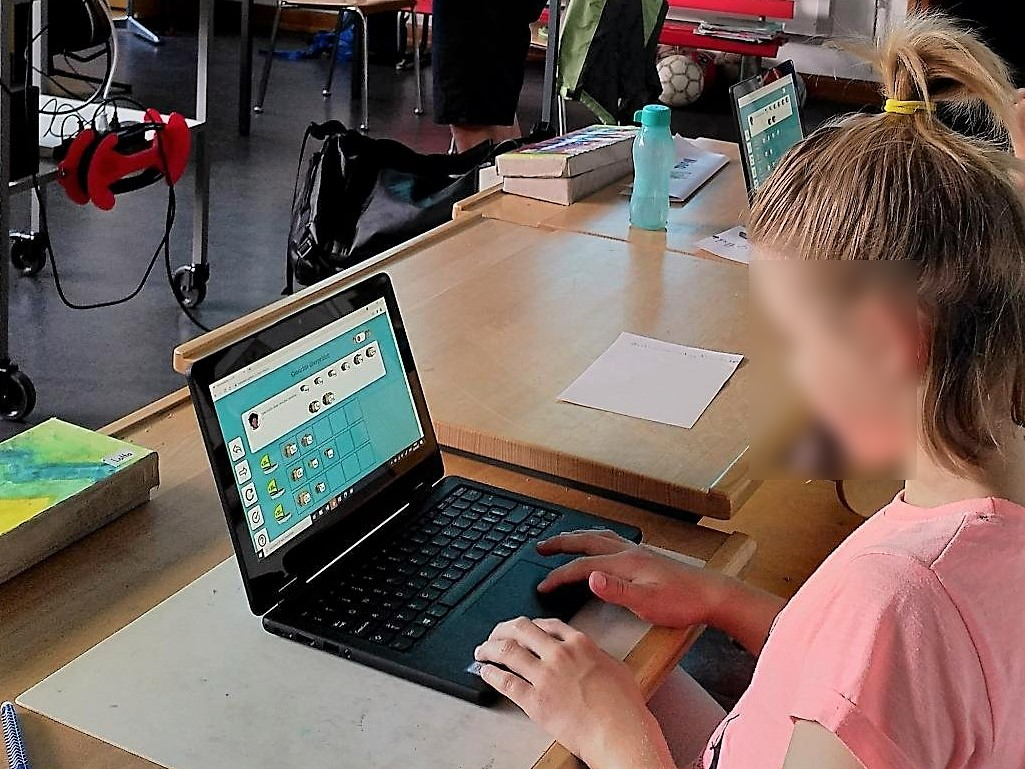
\includegraphics[width=1 \columnwidth]{figures/testing.png}
    \caption{Live testing in a third grade} 
    \label{fig:testing} 
\end{figure}

\subsection{Test Procedure}
The test was organized the following way: In the beginning, the project was presented and its vision and purpose was explained. Then, each student was provided a laptop or tablet and was instructed to solve problem instances for five to ten minutes for each different task type. Each student was advised to try to understand the exercise on their own and check the tutorial in case of problems. At the end, a quick feedback round was conducted, and each student had to fill out an online feedback form. Also, the link to the test website was distributed such that the students would be able to continue solving tasks at home and providing feedback if necessary.

\section{Test Results}
\label{section:results}

\subsection{Impressions and General Feedback}
The general impression of the live testing the teachers and test conductors had was surprisingly positive. The students were eager to solve the tasks and encouraged another to keep going. Some students were quick to understand the exercises and finished soon. Others needed some time to understand the concepts and rules and were not able so solve all the tasks. As for the randomly generated problem instances, some students continuously solved new challenges, while others got stuck with a single problem and needed help or additional explanations. As mentioned before, the range of tested students was very wide in terms of academic performance, such that a small fraction of students seemed unchallenged after a while when other students were overwhelmed with the amount and difficulty of the different task sets. These differences were to be expected, as in the case of the variety within the population. The impression of the testing is confirmed and backed up by some statistical data that will be presented in the next section.

\subsection{Data and Statistics}

The statistical feedback turned out to be thoroughly positive. The feedback form was designed the following way: First, the students had to provide some general information like the grade they attended at that time. The feedback form contained five major paragraphs, where the students had to describe their perception of the learning environment. The paragraphs included questions on how interesting the tasks were, how much fun it was to solve them, if the tasks were easy to understand, if the tutorial was being used and if the amount of exercises was satisfying. Some statistics are shown below to illustrate the feedback. For simplicity's and brevity's sake, only overall results are presented.

In the beginning, the platform had to be evaluated in terms of understandability and intuitiveness. The students were asked how long it took them to understand the exercises, and if they spent much time figuring out what the exact task description was. The result of the survey is visualized in figure \ref{fig:f1}.
Nearly all students considered the tasks to be intuitive and easy to understand. Only a few students did not understand the tasks and had to ask someone for help. These results line up with the impression of the test staff that had to guide single students to understand the requirements of the exercise.


\begin{figure}[H]
    \centering
    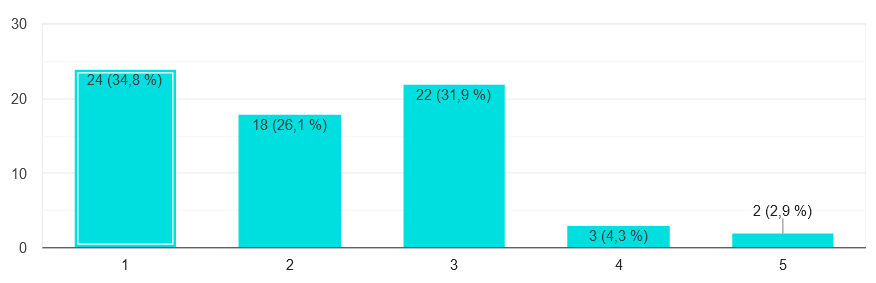
\includegraphics[width=1 \columnwidth]{figures/f1.png}
    \caption{Diagram - On a scale from 1 to 5, how hard were the exercises to understand? 1 corresponds to 'not very hard' and 5 to 'very hard'.} 
    \label{fig:f1} 
\end{figure}

Subsequently, the poll contained a question whether the students opened the tutorial often. This should  help on the one hand to ensure the correctness of the previous survey and on the other hand to know how the students approach a new, unknown task. Recall that the tutorial contains a text and tutorial video that can be opened if the task is unclear. The result of this poll is visualized in figure \ref{fig:f2} and confirmed the previous result that the tasks are well understandable. Additionally, it is evident that the students immediately try to solve the task by testing and trying out by themselves instead of reading the instructions. More than half of the students did not even look once at the tutorial, only few opened it regularly. This also lines up with the perception of the testing staff that noticed that some students did not even read the introductory sentence at the top of the exercise and instead immediately started clicking on the screen until they began to understand how to solve the problem instance.


\begin{figure}[H]
    \centering
    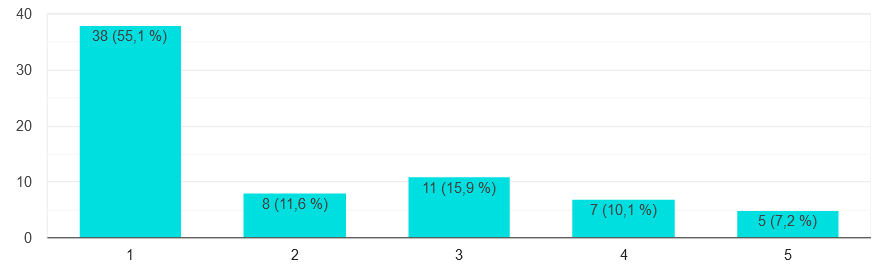
\includegraphics[width=1 \columnwidth]{figures/f2.png}
    \caption{Diagram - On a scale from 1 to 5, how often did you look at the tutorial? 1 corresponds to 'not very often' and 5 to 'very often'.} 
    \label{fig:f2} 
\end{figure}


Next, the satisfaction of the students was to be measured. The user was asked if he or she was content with the way the exercises are designed and if he or she liked the exercises. The result of this poll is visualized in figure \ref{fig:f3} and matched the general feedback of the students that they were very pleased with the learning platform. This was a highly recurring personal feedback among a majority of students. Over 80 percent of the students liked the tasks well to very well. Only a few did not like all of the exercises. An often mentioned reason for this answer was that the exercises were either too simple or too difficult to solve. This result was to be expected, as there are always a few students that are highly intelligent or have problems with reading and understanding assignments.

\begin{figure}[H]
    \centering
    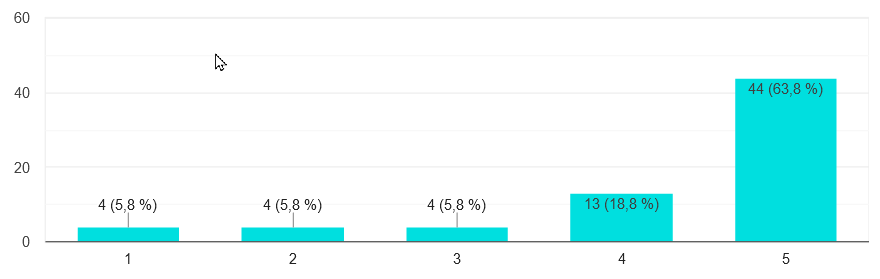
\includegraphics[width=1 \columnwidth]{figures/f3.png}
    \caption{Diagram - On a scale from 1 to 5, how much fun were the exercises? 1 corresponds to 'not so much fun' and 5 to 'much fun'.} 
    \label{fig:f3} 
\end{figure}

Another part of the questionnaire was a section on the attractiveness of the learning environment. The interviewed person had to evaluate how interesting and exciting the tasks were. The result of this poll can be found in figure \ref{fig:f4}. This result was relatively positive, since nearly 90 percent of the students thought the tasks were at least more or less interesting and overall nearly 40 percent rated the exercises to be highly fascinating.

\begin{figure}[H]
    \centering
    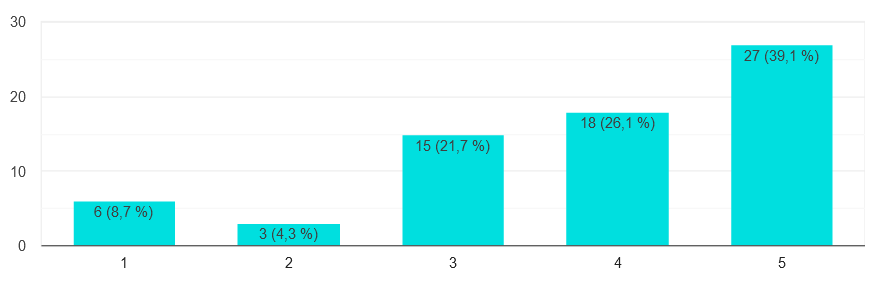
\includegraphics[width=1 \columnwidth]{figures/f4.png}
    \caption{Diagram - On a scale from 1 to 5, how interesting were the exercises? 1 corresponds to 'not very interesting' and 5 to 'very interesting'.}
    \label{fig:f4} 
\end{figure}

Besides this, a section was dedicated to measure the difficulty of the tasks. The user was asked how difficult the exercises were to solve and if the problems were challenging. Figure \ref{fig:f5} gives a detailed overview of the feedback data of this section. The results are as expected normally distributed, that is, there are students that could handle the tasks well while others were challenged by the different task sets. The perception of the task difficulty is normally distributed, with a small tendency towards easiness of the tasks.

\begin{figure}[H]
    \centering
    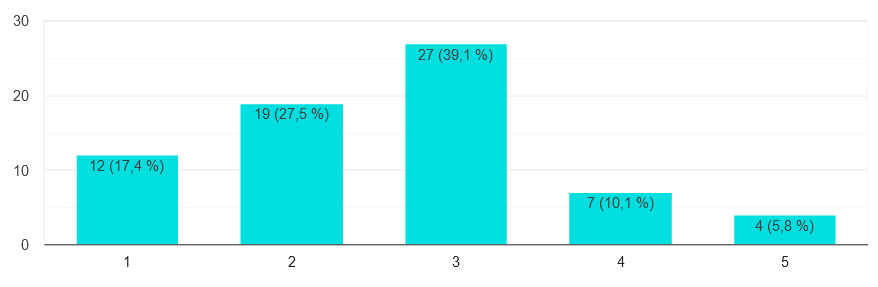
\includegraphics[width=1 \columnwidth]{figures/f5.png}
    \caption{Diagram - On a scale from 1 to 5, how hard were the exercises to solve? 1 corresponds to 'easy' and 5 to 'hard'.}
    \label{fig:f5} 
\end{figure}

In the final evaluation section, the students were asked if the amount of exercises was sufficient. The result of this poll is visualized in figure \ref{fig:f6}. About 3 out of 4 students were content with the variety of tasks.

\begin{figure}[H]
    \centering
    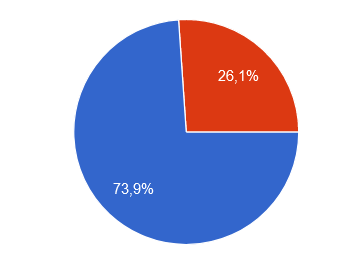
\includegraphics[width=0.5 \columnwidth]{figures/f6.png}
    \caption{Diagram - Are there enough different exercises in the learning environment?} 
    \label{fig:f6} 
\end{figure}
 
In every student feedback, there was then an additional section for written feedback on what one did or did not like and other comments. The results of this part do not deviate from the first five sections: Over 20 percent of the students remarked that they liked everything about the platform, while another 17 percent explicitly mentioned the task set on towers and 15 percent the kiosks task set. The exercises involving weights were mentioned by about 10 percent. Some students appreciated the fact that there are several difficulty levels. Furthermore, about 30 percent of the students explicitly wrote that there is nothing they did not like, while only a few feedbacks mentioned single details that could be improved.

This concludes the testing feedback. In the following, the next steps after the feedback evaluation will be laid out.

\section{Test Conclusion and Consequences}
\label{section:conclusion}

The test results confirmed the supervisor and expert feedback that the exercises are user-friendly and intuitive for elementary school students.

As a consequence of individual and statistical feedback, minor adaptions and corrections were made to the program code in order to enhance the user experience and functionality of the environment. The project could be completely revised and improved according to the feedback. In several task types, the tutorial was revised and extended such that the students can understand the exercise quicker. The introduction as well as the detailed explanation of the task were designed in a way that should even be more intuitive and easier to understand. 
Also, diverse game-play modifications were made to prevent the user from committing false steps in solving the problems. One student even discovered a small bug in the Tower game that allowed the user to place several towers on the same field, which could be immediately fixed. Other students explained what they did not find to be clear enough or what they did not understand at all. This way, real-life experience could be directly included, and the environment could be further enhanced.
%\input{sections/keepingSecret}
%\input{sections/learningFromData}
%\input{sections/representingInformation}
%\input{sections/testingAndCI}
\chapter{Conclusion}
\label{chapter:conclusion}
The objective of this bachelor thesis project was to build a learning environment for topics from the book 'einfach Informatik 3/4'. This goal to create a new platform has been achieved, and several games have been implemented. 

As for the first subtask \ref{subsection:t1}, the platform design and concept have been worked out and can be seen in the chapters on \nameref{chapter:design} and \nameref{chapter:concept}. For each task, a design was modelled, implemented and reviewed (see \nameref{chapter:weights}, \nameref{chapter:towers}, and \nameref{chapter:kiosks}).

The second point \ref{subsection:t2} could be adhered to, and the results and details can be found in the chapters on \nameref{chapter:design}, \nameref{chapter:architecture}, \nameref{chapter:testing} and in the learning environment itself. The most important requirement in the task description has been met, since the program is, as required, stable and works fluently on common operating systems.

Personally, my expectations were more than fulfilled. Arguably, the result of this Bachelor's thesis even succeeds my original plans. I'm very satisfied with the learning environment and thankful for the opportunity I received to implement commercial software. I learnt a lot with this project, and I am content with the overall outcome.

\section{Obstacles}
\label{section:obstacles}
In the beginning, the decisions concerning design and implementation techniques were a main obstacle. The details of the project were not fully clear (see chapter on \nameref{chapter:design}) and had to be worked out as a first step. As soon as the details were sorted out, the project could be organized, planned, and split up into single steps and intermediate goals.

Another obstacle that emerged was the implementation technique for \nameref{chapter:towers} and \nameref{chapter:kiosks} maps. The following fact brought several difficulties: There existed no fitting graph library with a graphical user interface such that created graphs can be displayed well. Furthermore, some existing graph libraries that met all requirements were either not well compatible or too expensive, so the choice was made to stick to fixed graphs that then had to be manually implemented. This turned out well, but was no easy assignment.

\section{Limitation}
\label{section:limitation}
In completing the fixture, it became clear that the number of tasks that can be implemented is limited by the short amount of time that is assigned to the Bachelor's thesis. 

In one design choice, the limitation of the project became particularly obvious. When implementing the task sets with towers and kiosks, the question arose whether a dynamic graph creator could be used. However, as mentioned before, several problems like compatibility, design and cost prevented its usage. 
As a consequence, graphs cannot be randomly created in this program and all maps had to be manually implemented. This heavily limits the scope of task instances and requires other approaches to provide a high number of exercises.


\section{Future Work}
\label{section:future}
The environment can be translated into various languages that then could be selected in the navigation bar. The underlying code concept enables the editor to simply add a new JSON file to add a new language to the learning environment (see section \ref{subsection:language}). 
Alternatively, more topics from the textbook 'einfach Informatik 3/4' could be implemented to further enlarge the variety of tasks. Especially, additional tasks containing graphs could be implemented, and the existing ones could be extended by a graph library.

Another next step could be to embed this learning environment into an even bigger learning platform, such that other chapters or even all topics of the textbook "einfach Informatik 3/4" can be covered. 

% This displays the bibliography for all cited external documents. 
% All references have to be defined in the file references.bib and can then be cited from within this document.
\bibliographystyle{IEEEtran}
\bibliography{references}

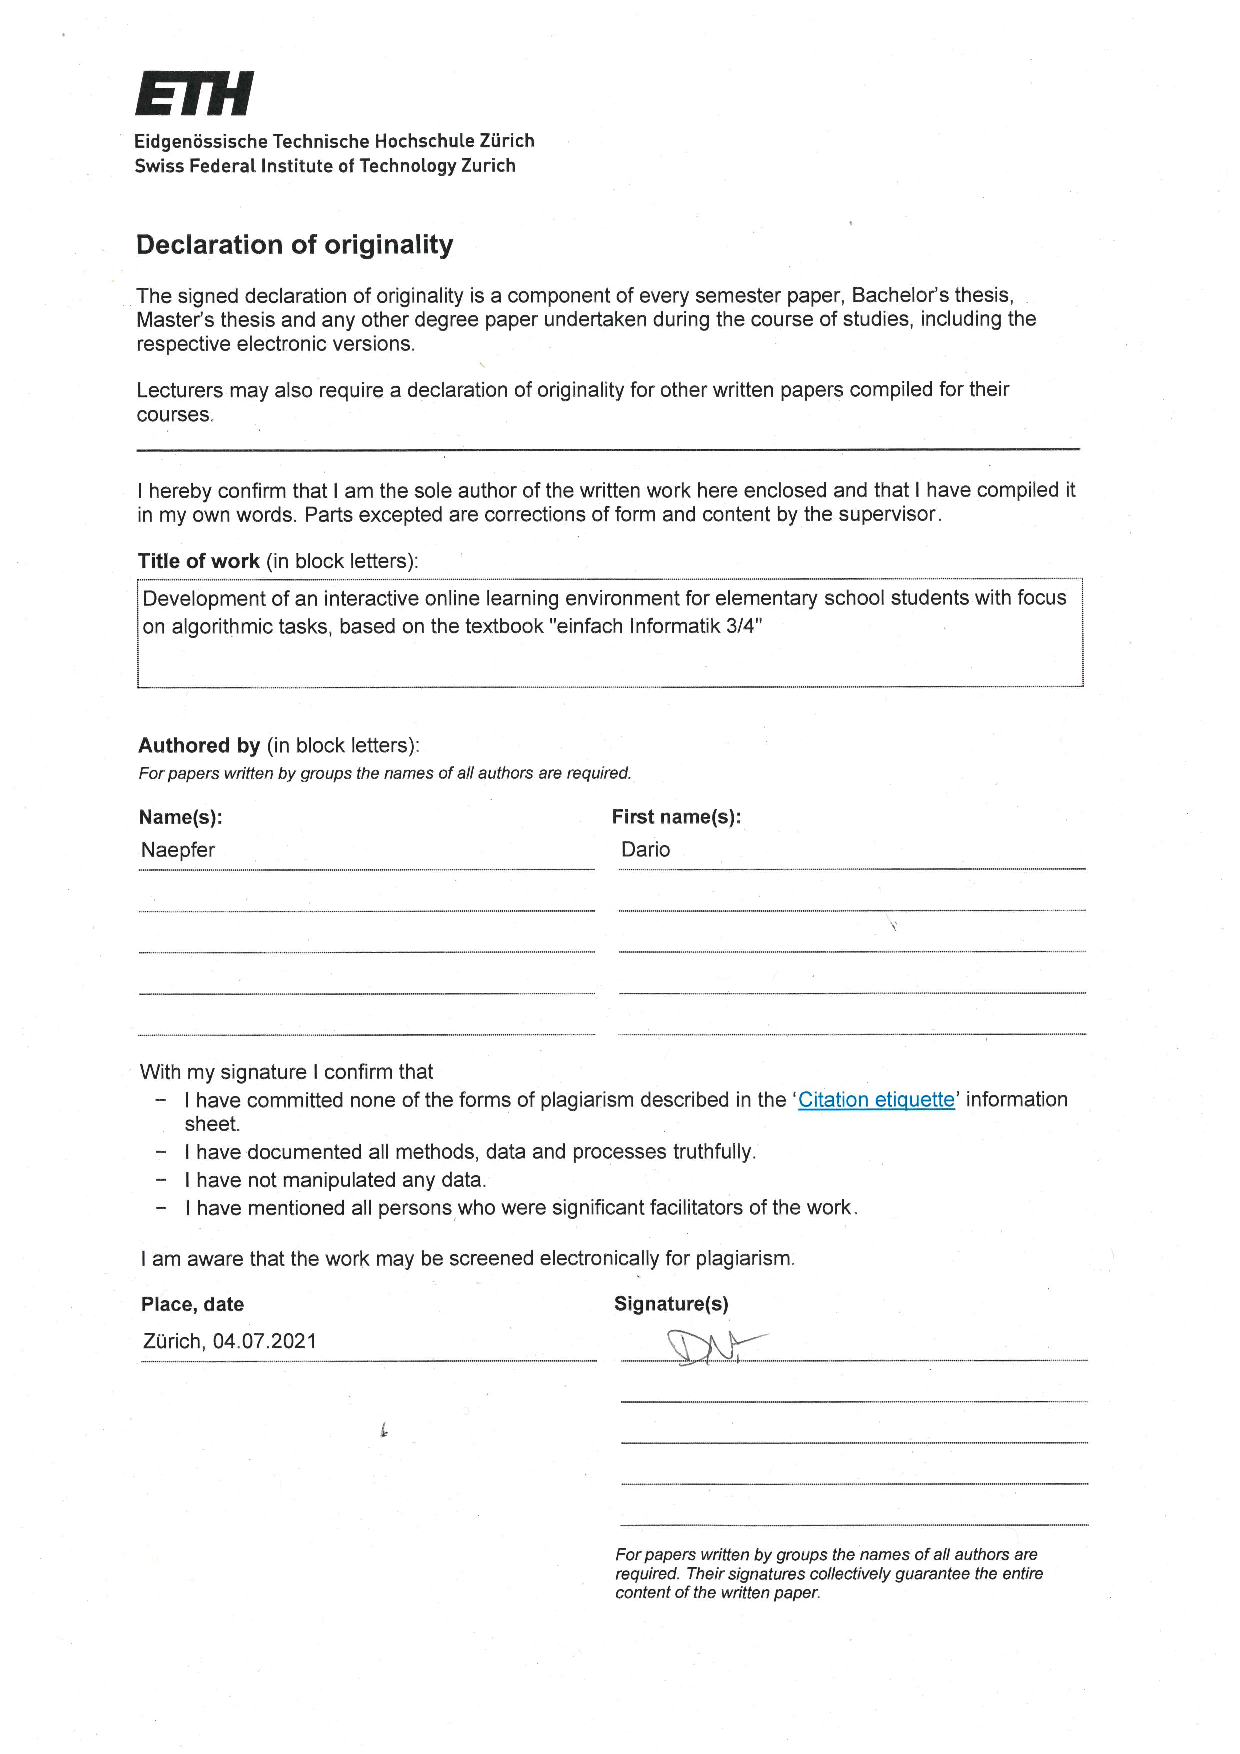
\includepdf[pages={1-},scale=1]{pdf/originality.pdf}

% This creates an appendix chapter, comment if not needed.
% \appendix
% \input{appendix/example}

\end{document}